\documentclass[12pt]{uconnthesis}
% You can choose 10pt, 11pt or 12pt as font size.

% \let\emph\relax
% \DeclareTextFontCommand{\emph}{\bfseries}
\DeclareEmphSequence{\textbf}
% Draft Versions : Uncomment this if you want to see the name of labels that you declare.
%\usepackage{showkeys}  

% Always keep the settings and the definitions
%%
%% BOF settings.tex
%%


%%
%% MARGIN DECLARATIONS
%%
%% The Graduate School requires the following minimal margins: 1in on top, right and bottom 
%% and 1.5in on the left. And yes, this feature, they check.
          
\voffset -15mm
\hoffset 2mm
\setlength{\textheight}{220mm}
\setlength{\textwidth}{145mm}


%%
%% LaTeX EXTENSIONS
%%

% Most of these packages are not needed for the UConn Thesis class, but are quite useful
% for writing your thesis. Documentation about these packages can be found in your
% average LaTeX manual or by doing the following Google search :
% "latex <name-of-the-package> documentation site:www.tug.org" 

\usepackage{amsmath} % AMS math commands like \frac{}{} 
\usepackage{amscd} % commutative diagrams made easy -  has to be loaded after amsmath
\usepackage{amsthm}  % theorem, lemma, definition, ... -  has to be loaded after amsmath
\usepackage{calc} % minimal calculator operations

\usepackage{graphicx} % Imports figures : pdf, jpg, png, tif (one f)
                      % Use the package graphics if you use eps files.
                      % Warning : It is very difficult to use both graphics and graphicx.

% \usepackage{enumerate} % extends enumerate environment
\usepackage{dsfont, marvosym, latexsym, amssymb, wasysym, mathbbol} % extra symbols 
\usepackage{color} % use colors red/blue/green/yellow/magenta
\usepackage{fancyhdr} % headers
\usepackage{fancybox} % oval boxes and stuff
\usepackage{ifthen} % if-then-else structure
\usepackage{rotate} % rotate and mirror commands

% Caligraphic Alphabet - used by the definitions of \cA, \cB, \cC and so on.
\usepackage[mathcal]{euscript}       
% Very Curly Caligraphic Alphabet - used by the definitions of \ccA, \ccB, \ccC and so on.
\usepackage{mathrsfs}       

%%
%% FONT DECLARATIONS
%%

% There are many fonts out there for LaTeX. If you want to see what your thesis looks like
% in this font, uncomment one of them. If all of them remain inactive, the system default will
% be chosen (usually Courier). A few warnings:
% (a) The Graduate School wants the fonts to be simular to Times New Roman, Helvetica or Arial.
%     Yes, Courier is fine. As you will notice many of the options below are only slightly different.
%     Of these fonts, cmbright and pxfonts are slightly outlandish and bookman is somewhat (too?) heavy.
% (b) Changeing from one font to another can give (rather small) changes in layout.
% (c) Some of these declarations need LaTeX extensions, so don't move this section before the previous one. 
%
% Choose one of the following:
% avant, bookman, charter, cmbright, courier, helvet, newcent, times, palatino, pxfonts

\usepackage{times}

%%
%% JASPER'S PACKAGES
%%
\usepackage{amsrefs} % ams style references
\newcommand{\description}{} % necessary for some reason
\usepackage{enumitem} % better than enumerate
\usepackage{ulem} % strikeout and various underline types
\usepackage{tikz} % tikz figures
\usepackage{mathtools} % mathclap primarily
\usepackage{hyperref} % in-document hyperlinks

%%
%% DEF. THM. LEMMA AND THE REST 
%%

% Comment the following line out if you want "Theorem 1.2.3" and not "1.2.3 Theorem"
% \swapnumbers 

% Equations will be numbered with their section number, i.e. (1.1.1), (1.1.2), (1.2.1) and so on.
% Commenting this out put will result in all equations being numbered (1), (2), (3), ... (999) which
% is not the best idea for a document as long as a thesis.
\numberwithin{equation}{section}                      

% There are three theoremstyles: plain, definition and remark.
% Notice that "definition" produces the most standard output.
\theoremstyle{definition}

% If you want to use subsections, change the word "section" to "subsection" in the following declaration.
% however, be advised that then all numbering labels will contain 4 numbers and that you should divide
% up _every_ section into subsections or get labels like (2.2.0.1), (2.2.0.2), (2.2.0.3) etc.
\newtheorem{theorem}{Theorem}[section]

% These commands use the amsthm package. If you want to add a declatarion, it has to be of the form
% \newtheorem{environment-name}[theorem]{Word-you-want-printed}
\newtheorem{definition}[theorem]{Definition}
\newtheorem{definitions}[theorem]{Definitions}
\newtheorem{lemma}[theorem]{Lemma}
\newtheorem{myexample}[theorem]{Example}
\newtheorem{myexamples}[theorem]{Examples}
\newtheorem{proposition}[theorem]{Proposition}
\newtheorem{property}[theorem]{Property}
\newtheorem{properties}[theorem]{Properties}
\newtheorem{corollary}[theorem]{Corollary}
\newtheorem{notation}[theorem]{Notation}
\newtheorem{notations}[theorem]{Notations}
\newtheorem{remark}[theorem]{Remark}
\newtheorem{remarks}[theorem]{Remarks}
\newtheorem{introduction}[theorem]{Introduction}
\newtheorem{framework}[theorem]{Framework}
\newtheorem{conditions}[theorem]{Conditions}

% Jasper's theorem commands
\newtheorem{myclaim}[theorem]{Claim}

% The Q.E.D. symbol can be defined in any way.  
% Commenting this out will give the default which is an empty square.
% \renewcommand{\qedsymbol}{{\slshape Qed}}


%%
%% PARINDENT 0
%%

% Needed to keep titles of Section and Subsections in their place,
% amongst other reasons. Do not change.
\parindent 0pt 


%%
%% DEFAULT ENUMERATE FORMATS
%%

\renewcommand\theenumi{\roman{enumi}}
\newcommand\labelenumi{(\theenumi)\ \ }
\renewcommand\theenumii{\alph{enumii}}
\newcommand\labelenumii{(\theenumii)\ }
\renewcommand\theenumiii{\roman{enumiii}}
\newcommand\labelenumiii{(\theenumiii)\ }
\renewcommand\theenumiv{\Alph{enumiv}}
\newcommand\labelenumiv{(\theenumiv)\ }
\leftmargini 30pt 
\leftmarginii 15pt 
\leftmarginiii 15pt 
\leftmarginiv 10pt 
\labelsep 5pt


%%
%% DEFAULT ITEMIZE FORMATS
%%

\newcommand\labelitemi{\textbullet}
\newcommand\labelitemii{\normalfont\bfseries\textendash}
\newcommand\labelitemiii{\textasteriskcentered}
\newcommand\labelitemiv{\textperiodcentered}


%%
%% EOF settings.tex
%%


%%
%% JASPER'S COMMANDS
%%

\newcommand{\RR}{\mathbb{R}} % Real numbers
\newcommand{\CC}{\mathbb{C}} % Complex numbers
\newcommand{\NN}{\mathbb{N}} % Natural numbers
\newcommand{\PP}{\mathbb{P}} % Projective Space
\newcommand{\re}{\text{Re}~} % Real part
\newcommand{\im}{\text{Im}~} % Imaginary part

\def\mclimits_#1{\limits_{\mathclap{#1}}} % Collapsable limits
%%
%% BOF definitions.tex
%%


%%
%% BASIC FONT DECLARATIONS
%%
%% These shorthands are usually declared by the class 'article.cls' or 'book.cls'
%% As we are not in such a class, we have to declare them ourselves.

\def\it{\itshape}
\def\sl{\slshape}
\def\sc{\scshape}
\def\tt{\texttt}
\def\bf{\textbf}
\def\rm{\rmdefault}


%%
%% DOUBLE LEFT LINE LETTERS
%%

\def\IE{\hbox {I \hskip -5.2pt {E}}}
\def\IP{\hbox {I \hskip -5.2pt {P}}}

\def\IR{\mathbb{R}}
\def\IQ{\mathbb{Q}}
\def\IN{\mathbb{N}}
\def\IK{\mathbb{K}}
\def\I1{\mathbb{1}}
\def\IC{\mathbb{C}}
\def\IS{\mathbb{S}}
\def\ZZ{\mathbb{Z}}


%%
%% CALIGRAPHIC ALPHABET
%%
%% This is a caligraphic alphabet slightly curlier than with the standard {\cal A} command.

\def\cA{\mathcal{A}}
\def\cB{\mathcal{B}}
\def\cC{\mathcal{C}}
\def\cD{\mathcal{D}}
\def\cE{\mathcal{E}}
\def\cF{\mathcal{F}}
\def\cG{\mathcal{G}}
\def\cH{\mathcal{H}}
\def\cI{\mathcal{I}}
\def\cJ{\mathcal{J}}
\def\cK{\mathcal{K}}
\def\cL{\mathcal{L}}
\def\cM{\mathcal{M}}
\def\cN{\mathcal{N}}
\def\cO{\mathcal{O}}
\def\cP{\mathcal{P}}
\def\cQ{\mathcal{Q}}
\def\cR{\mathcal{R}}
\def\cS{\mathcal{S}}
\def\cT{\mathcal{T}}
\def\cU{\mathcal{U}}
\def\cV{\mathcal{V}}
\def\cW{\mathcal{W}}
\def\cX{\mathcal{X}}
\def\cY{\mathcal{Y}}
\def\cZ{\mathcal{Z}}


%%
%% VERY CALIGRAPHIC ALPHABET
%%
%% This caligraphic alphabet is quite curly. Don't use this one if you have thirty or so symbols of it on
%% one page. Thechnically there's no problem, but it will look a little overdone in that case.

\def\ccA{\mathscr{A}}
\def\ccB{\mathscr{B}}
\def\ccC{\mathscr{C}}
\def\ccD{\mathscr{D}}
\def\ccE{\mathscr{E}}
\def\ccF{\mathscr{F}}
\def\ccG{\mathscr{G}}
\def\ccH{\mathscr{H}}
\def\ccI{\mathscr{I}}
\def\ccJ{\mathscr{J}}
\def\ccK{\mathscr{K}}
\def\ccL{\mathscr{L}}
\def\ccM{\mathscr{M}}
\def\ccN{\mathscr{N}}
\def\ccO{\mathscr{O}}
\def\ccP{\mathscr{P}}
\def\ccQ{\mathscr{Q}}
\def\ccR{\mathscr{R}}
\def\ccS{\mathscr{S}}
\def\ccT{\mathscr{T}}
\def\ccU{\mathscr{U}}
\def\ccV{\mathscr{V}}
\def\ccW{\mathscr{W}}
\def\ccX{\mathscr{X}}
\def\ccY{\mathscr{Y}}
\def\ccZ{\mathscr{Z}}


%%
%% LOGICAL OPREATORS
%%

\def\myOR {\ \ \ {\tt OR} \ \ \ }
\def\myAND {\ \ \ {\tt AND} \ \ \ }
\def\myand {\ \hbox{and}\ }
\def\myor {\ \ \ \hbox{or} \ \ \ }


%%
%% LIMITS AND SUMS
%%

\def\limn{\lim_{n \to \infty}}
\def\limk{\lim_{k \to \infty}}
\def\limh{\lim_{h \to 0}}
\def\limxinf{\lim_{x \to \infty}}
\def\limninf{\lim_{n \to +\infty}}
\def\limxc{\lim_{x \to c}}
\def\limxalpha{\lim_{x \to \alpha}}
\def\limx0{\lim_{x \to 0}}
\def\sumkn{\sum_{k=0}^n}
\def\sumkinfty{\sum_{k=0}^{\infty}}
\def\sumninfty{\sum_{n=0}^{\infty}}
\def\sumid{\sum_{i=1}^{d}}
\def\sumijd{\sum_{i=1, j=1}^{d}}


%%
%% FUNCTIONS
%%

\def\e{\hbox{e}}
\def\cosec{\hbox{cosec}}
\def\cotan{\hbox{cotan}}
\def\cotg{\hbox{cotg}}
\def\arccot{\hbox{arccot}}
\def\arcsec{\hbox{arcsec}}
\def\arccosec{\hbox{arccosec}}
\def\arcsinh{\hbox{arcsinh}}
\def\arccosh{\hbox{arccosh}}
\def\arctanh{\hbox{arctanh}}
\def\arccoth{\hbox{arccoth}}


%%
%% PROBABILITY
%%

\def\erf{\hbox{erf}}
\def\indicator#1{\mathbb{1}_{\{ #1\} }}
\def\process#1#2{\{#1_{#2}\}_{#2}}


%%
%% DERIVATIVES
%%

\def\ddx#1{\frac{d{#1}}{dx}}
\def\pdd#1#2{\frac{\partial {#1}}{\partial {#2}}}
\def\pddtwo#1#2#3{\frac{\partial^2 {#1}}{\partial {#2} \partial {#3}}}


%%
%% INTEGRALS
%%

\def\intinfinf{\int_{-\infty}^{+\infty}}
\def\intoinf{\int_{0}^{+\infty}}
\def\intunitball{\underset{\| x \| \leq 1}{\int}}
\def\intxyleq1{\underset{\| x - y  \| \leq 1}{\int}}
\def\intxygeq1{\underset{\| x - y  \| \geq 1}{\int}}
\def\intxizetaleq1{\underset{\| \xi - \zeta  \| \leq 1}{\int}}
\def\intxizetageq1{\underset{\| \xi - \zeta \| \geq 1}{\int}}
\def\intA{\underset{A}{\int}}
\def\intRd{\underset{\IR^d}{\int}}
\def\intt{\int_0^t\!\!}
\def\doubleint#1{\int\limits_{#1}\!\!\!\!\int}
\def\tripleint#1{\int\!\!\!\!\int\limits_{#1}\!\!\!\!\int}


%%
%% IR^d
%%

\def\point#1#2{\left({#1}_1 , \ldots , {#1}_{#2}\right)}
\def\vector#1#2{\left<{#1}_1 , \ldots , {#1}_{#2}\right>}
\renewcommand{\vec}{\overrightarrow}


%%
%% SKIP & CO
%%

\def\standardskip{\vskip 3mm}
\def\miniskip{\vskip 2mm}
\def\hyperquad{\quad\quad\quad\quad}


%%
%% PUTDATE
%%
%% Call \putdate at the beginning of a chapter. Then you know when the printout was compiled.

\newcounter{hours}
\newcounter{minutes}
\newcommand\printtime{%
  \setcounter{hours}{\the\time/60}%
  \setcounter{minutes}{\the\time-\value{hours}*60}%
  \ifthenelse{\value{hours} > 12}
     {
       \setcounter{hours}{\value{hours}-12}%
       \thehours:\theminutes \ p.m.                
     }
     {
       \thehours:\theminutes \ a.m.                
     } 
}

\def\putdate{{\tt Compiled on \the\month-\the\day-\the\year \ at\printtime} \\}


%%
%% MISCELLANEOUS
%%

\def\rmin{{r\hbox{-}}}
\def\smin{{s\hbox{-}}}
\def\tmin{{t\hbox{-}}}

\def\cadlag{\hbox{c\`adl\`ag }}

\def\inproduct#1#2{\langle ~ {#1} ~ | ~ {#2} ~ \rangle}

\def\longto{\longrightarrow}
\def\halflambda{{\scriptstyle\frac{\lambda}{2}}}

\def\realline#1#2{ \[
                     \begin{CD}
                     {\hskip #1mm} @<<<${\hskip -12mm}$@>{\hskip #2mm}>>\\
                     \end{CD}
                     \]
                   }

\def\ovalbox#1#2{
       \begin{flushright}
       \Ovalbox{ 
           \begin{minipage}{#1}
             #2
           \end{minipage}
         }
       \end{flushright}
       }

\def\mystretch{\ensuremath{\phantom{\displaystyle\int\limits_X}}}


%%
%% SPECIFIC Marc Corluy
%%

\def\intrS{\int\limits_0^r\!\!\!\int\limits_S}
\def\intsS{\int\limits_0^s\!\!\!\int\limits_S}
\def\inttS{\int\limits_0^t\!\!\!\int\limits_S}
\def\intrD{\int\limits_0^r\!\!\!\int\limits_D}
\def\intsD{\int\limits_0^s\!\!\!\int\limits_D}
\def\inttD{\int\limits_0^t\!\!\!\int\limits_D}

\def\sumid{\sum_{i=1}^d}
\def\sumjd{\sum_{j=1}^d}
\def\sumkd{\sum_{k=1}^d}
\def\sumijd{\sum_{i,j=1}^d}
\def\sumkld{\sum_{k,l=1}^d}
\def\sumz{\sum_{z \in \ZZ^d}}

\def\Cxhz{C_{\frac{x}{h},\frac{x}{h}+z}}
\def\Cyhz{C_{\frac{y}{h},\frac{y}{h}+z}}
\def\tCxhz{{\tilde C}_{\frac{x}{h},\frac{x}{h}+z}^{\varepsilon}}

\def\tX{\tilde X}

\def\Jumpp{\Gamma}

%%
%% EOF definitions.tex
%%


% Only activate the parts that you want to compile. You might want
% to go chapter by chapter. Keep the bibliography included, because 
% you will probably refer to it in every chapter.

% If you don't have a notationpage, comment it out.

% If you don't want a chapter that says "Introduction" instead of "Chapter 1",
% comment out the line with introchapter.

\includeonly{
  front_matter,
  notationpage,
  introchapter,
  chapter1,
  chapter2,
  chapter3,
  % chapter4,
  % chapter5,
  % chapter6,
%  chapter7,
%  chapter8,
%  appendixa,
%  appendixb,
%  appendixc,
%  appendixd, 
  bibliography
}


\begin{document}

%%
%% BOF front_matter.tex
%%


%%
%% THESIS TITLE
%%

\myThesisTitle{Rates of Convergence in the Central Limit Theorem for Markov Chains}


%%
%% PERSONAL DATA
%%

\myName{Your Name Goes Here}

\myNewDegreeShort{Ph.D.}
\myNewDegreeLong{Doctor of Philosophy}

\myPreviousDegreeShort{M.Sc. Math., M.Sc. Th.Phys.}
\myPreviousDegreeLong{
  M.Sc. Mathematics, Universiteit Antwerpen, Antwerp, Belgium, 1992 \\
  M.Sc. Theoretical Physics, Universit\'e Libre de Bruxelles, Brussels, Belgium, 1993
}


%% 
%% ADVISORS
%%

% Fill in your advisors. Comment out the last ones if you have less than 4 Associate Advisors.

\myMajorAdvisor{Richard Bass}
\myAssociateAdvisorA{Evarist Gin\'e-Masd\'eu}
\myAssociateAdvisorB{Yung-Sze Choi}
%\myAssociateAdvisorC{Advisor C}
%\myAssociateAdvisorD{Advisor D}


%%
%% TABLE OF CONTENTS               
%%

% This variable determines what will be in the Table of Contents
% 0 = Chapters only, 1 = Chapters and Sections, 2 = Chapters, Sections and Subsections
% If not set, the default will be "2", i.e. the titles of Chapters, Sections and 
% Subsections will be displayed in the table of contents.
\myTOCDepth{2}


%%
%% ABSTRACT PAGE , TITLE PAGE 
%%

% These pages will not be numbered. The abstract will always be double spaced. 
% If the abstract runs on to a second pages, then this page will be headed as follows:
% <myName> - University of Connecticut - <thisYear>

\begin{abstractpage}
Put your abstract here. Try to use as little symbols as possible. This abstract will be typeset 
for web publishing and various databases (not by you), and symbols don't transfer well.
\end{abstractpage}

\begin{titlepage}
  % Leave this blank.
\end{titlepage}


%%
%% THE REST OF THE FRONT MATTER PAGES
%%

% Copyright, Approval, Dedication, Acknowledgments,
% Table of Contents, List of Figures, List of Tables
% Comment out those that you don't need.
% These pages are numbered with lowercase Roman numerals.

\begin{romanpages}

\begin{copyrightpage}
  % Leave this blank.  
\end{copyrightpage}

\begin{approvalpage}
  % Leave this blank.  
\end{approvalpage}

% \begin{dedicationpage}
%  If you want to dedicate your thesis to someone / something, put the dedication here.
%  If not, comment both \begin{dedicationpage} and \end{dedicationpage} out. 
% \end{dedicationpage}

\begin{acknowledgementpage}
At this point, I would like to thank the many people who - directly or indirectly - have contributed
to this dissertation. .........\\
\end{acknowledgementpage}


% This Page will automatically generate a table of contents.
\begin{contentpage}
  \begin{flushleft}
    % comments between the title and the table, if any.                
  \end{flushleft}
  \tableofcontents
  \begin{flushleft}
    % comments after the table, again, if any.
  \end{flushleft}
\end{contentpage}

% This page will automatically generate a list of figures.
% If you don't have any figures, leave it commented out.
%\begin{figurepage}
%  \begin{flushleft}
%    comments between the title and the table, if any.
%  \end{flushleft}
%  \listoffigures
%  \begin{flushleft}
%    comments after the table, again, if any.
%  \end{flushleft}
%\end{figurepage}

% This page will automatically generate a list of tables.
% If you don't have any tables, leave it commented out.
%\begin{tablepage}
%  \begin{flushleft}
%    comments between the title and the table, if any.
%  \end{flushleft}
%  \listoftables
%  \begin{flushleft}
%    comments after the table, again, if any.
%  \end{flushleft}
% \end{tablepage}

\end{romanpages}

%%
%% EOF front_matter.tex
%%

\begin{notationpage}

\vskip 15mm

(This section should be for reference only and most of these symbols should be defined in the text)
% \begin{enumerate}[label=\alph*)]
%   \item Multiindex notation
%   \begin{itemize}
%     \item $x^\alpha = x_1^{\alpha_1}x_2^{\alpha_2} \cdots x_n^{\alpha_n}$ with $0^0 = 1$ when necessary.
%     \item $\binom{k}{\alpha} = \frac{k!}{\alpha_1!\alpha_2!\cdots\alpha_n!}$
%   \end{itemize}
% \end{enumerate}

First recall the conventional multiindex notation. Let $\NN_0$ denote the nonnegative integers. A multiindex $\alpha = (\alpha_1, \alpha_2, \ldots, \alpha_n) \in \NN_0^n$ is an $n$-tuple of nonnegative integers. The degree of a multiindex is $|\alpha| = \alpha_1 + \alpha_2 + \cdots + \alpha_n$. Multivariate exponentiation is defined as follows. For $x = (x_1, x_2, \ldots, x_n) \in \RR^n$,
\[
  x^\alpha = x_1^{\alpha_1}x_2^{\alpha_2} \cdots x_n^{\alpha_n}.
\]
Here we will use the convention $0^0 = 1$ so that for example ${(x, y, z)}^{(0, 1, 0)} = y$. We will use $e_i \in \RR^n$ to represent the canonical unit vector
\[
  e_i = (0, \ldots, 0, 1, 0, \ldots, 0)
\]
which can also be interpreted as a multiindex so for example
\[
  (x,y,z)^{2e_1 + e_3} = x^2z
\]

The multinomial formula gives a convenient expansion for multinomial powers. Let $k \in \NN_0$. Then
\[
  {(b_1 + b_2 + \cdots + b_n)}^k = \sum_{|\alpha| = k} \binom{k}{\alpha} b^\alpha
\] 
where the multinomial coefficients are defined
\[
  \binom{k}{\alpha} = \frac{k!}{\alpha_1! \alpha_2! \cdots \alpha_n!}.
\]
Note that the multinomial expansion sums over all multiindeces $\alpha \in \NN_0^n$ of degree $k$.

We denote the standard euclidean inner product
\[
  \langle x,y \rangle = x_1y_1 + x_2y_2 + \cdots + x_n y_n
\]
where $y = (y_1, y_2, \ldots, y_n) \in \RR^n$ and the Euclidean norm 
\[
  \|x\| = \sqrt{x_1^2 + x_2^2 + \cdots + x_n^2}
\]
We may slightly abuse notation by using the inner product and norm in different dimensions, even in the same equation. This can be excused if one views each euclidean space $\RR^n$ as embedded in the sequence space $\ell^2(\RR^\NN)$ in which the inner product and norm are equivalent.

When discussing hyperplanes in $\RR^n$ we index them by a unit normal vector, $\omega \in S^{n-1}$, and distance from origin $-\infty < p < \infty$, and we write for example the implicit hyperplane equation $\langle x, \omega \rangle = p$. Note that $\langle x, -\omega \rangle = -p$ represents the same hyperplane. It is perhaps more correct, in later defining the Radon and Gaussian Radon transforms, to identify these indexes and define the transforms over a projective space. We omit this discussion as it is not relevant within the scope of this work.
\begin{figure}[h]
  \centering
  \begin{tikzpicture}[plane/.style={<->,thick,blue},
        vector/.style={->,red},
        axis/.style={->,black}]
    %draw axes
    \draw[axis] (-1,0) -- (3,0) node[anchor=west]{$x_1$};
    \node at (-.2,.2) {$\mathbf{0}$};
    \draw[axis] (0,-1) -- (0,3) node[anchor=west]{$x_2$};
    %draw plane
    \draw[plane] (-1, 3) -- (3, -1) node[midway, right]{~$\langle x, \omega\rangle = p$};
    %draw projection angle and orthogonal vector
    \draw[red,dashed] (-1,-1) -- (3,3);
    \def\ra{.07};
    \draw[red] (1-\ra, 1-\ra) -- (1,1-2*\ra) -- (1+\ra,1-\ra);
    \draw[vector] (0,0) -- (0.7,0.7) node[above left]{$\omega$};
    %draw extension line
    \draw[very thin, red] (\ra, -\ra) -- (1+\ra, -1-\ra);
    \draw[<->,very thin, red] (1+\ra, -1-\ra) -- (2+\ra, -\ra) node[midway,below right]{$p$};
  \end{tikzpicture}
  \caption{Hyperplane equation}\label{fig:HypEq}
\end{figure}

Unless otherwise indicated all measures are Euclidean measures, that is the Borel measure assocciated with the standard Euclidean metric on a given space. In particular the Euclidean measure on a hyperplane of $\RR^n$ is equivalent to the Euclidean measure on $\RR^{n-1}$. We chose for convenience to denote measures by their associated variable such as $dx$, $dp$, $dz$, and others. It should be stated that this notation, while uniform, is context dependent. For example in the integrals
\[
  \int_{\RR^n}~dx \qquad \text{and} \qquad \int_{\langle x, \omega\rangle = p} ~dx,
\]
the measure $dx$ is to be understood as the $n$-dimensional and $(n-1)$-dimensional Euclidean measure respectively.

% \begin{enumerate}[A) ]

%   \item \bf{Spaces}       
%         \begin{itemize}
%           \item $\ccL^2(\IR^d)$, all square integrable functions.
%           \item $\ccD(\IR^d)$, all cadlag functions.
%           \item $\ccC(\IR^d,\IR)$, all continuous functions from $\IR^d$ to $\IR$.
%           \item $\ccC_0(\IR^d,\IR)$, those functions in $\ccC(\IR^d,\IR)$ that vanish at infinity.
%           \item $\ccC_{00}(\IR^d,\IR)$, those functions in $\ccC(\IR^d,\IR)$ that have compact support.        
%         \end{itemize}
%         \vskip 1mm          

%   \item \bf{General Operators}       
%         \begin{itemize}
%           \item $\cL$, $\cM$, $\hat\cL$, $\hat\cM$ : generators of a semigroup
%           \item $\cP_t$, $\cQ_t$, $\hat\cP_t$, $\hat\cQ_t$ : the corresponding semigroups                    
%         \end{itemize}
%         \vskip 1mm          

%   \item \bf{Specific Operators}   
%         \begin{itemize}
%           \item $Lf(x) = \nabla \cdot A(x) \nabla ~ f (x)$
%           \item $\tilde Lf(x) = \nabla \cdot \tilde A(x) \nabla ~ f (x)$
%           \item $L^h f(x) = \frac{1}{h^2} ~ \sum\limits_{z \in \ZZ^d} (f(x+hz)-f(x)) ~ \Cxhz$
%           \item $\tilde L^h f(x) = \frac{1}{h^2} ~ \sum\limits_{z \in \ZZ^d} (f(x+hz)-f(x)) ~ \tCxhz$
%           \item Semigroups: $P_t = e^{tL}$, $\tilde P_t = e^{t\tilde L}$, 
%                 $P_t^h = e^{tL^h}$, $\tilde P_t^h = e^{t\tilde L^h}$
%         \end{itemize}
%         \vskip 1mm          

%   \item \bf{Markov Processes}
%         \begin{itemize}
%           \item $X_t^{(h)}$ is the process on $h\ZZ^d$ with generator $L^h$. 
%           \item $\tilde X_t^{(h)}$ is the process on $h\ZZ^d$ with generator $\tilde L^h$. 
%           \item $X_t$ is the process on $\IR^d$ with generator $L$. 
%           \item $\tilde X_t$ is the process on $\IR^d$ with generator $\tilde L$. 
%         \end{itemize}

%   \mynewpage{1}

%   \item \bf{Dirichlet Forms} \\
%         In general, $\ccE_\cM(f,g) = - \langle \cM f | g \rangle$. In $\ccL^2 (\IR^d,\mu)$, the
%         inner product is defined as
%         \begin{equation*}
%           \langle  f | g \rangle = \int\limits_{\IR^d} f(x) g(x) dx
%         \end{equation*}
%         while in $\ccL^2 (h\ZZ^d,\mu^h)$ it is defined as
%         \begin{equation*}
%           \langle  f | g \rangle = h^d ~ \sum\limits_{x \in h\ZZ^d} f(x) g(x)  .                           
%         \end{equation*}
%         Note the rescaling factor $h^d$. Therefore, the various Dirichlet forms are
%         \begin{itemize}
%           \item $\ccE(f,g) = - \displaystyle\int [\nabla \cdot A \nabla ~ f](x) ~ g(x) ~ dx$
%           \item $\tilde \ccE(f,g) = - \displaystyle\int [\nabla \cdot \tilde A \nabla ~ f](x) ~ g(x) ~ dx$
%           \item $\ccE^h(f,g) = \frac{1}{2} ~ h^{d-2}                 
%                                   ~\sum\limits_{x,z \in \ZZ^d} (f(x+hz)-f(x))~(g(x+hz)-g(x)) ~\Cxhz$               
%           \item $\tilde \ccE^{h,\varepsilon} (f,g) = \frac{1}{2} ~ h^{d-2} ~ \sum\limits_{x,z \in \ZZ^d} 
%                                         (f(x+hz)-f(x)) ~ (g(x+hz)-g(x)) ~ \tCxhz$                      
%         \end{itemize}
%         \vskip 1mm          

%   \item \bf{Our Standard Mollifier} \\
%         For each $\varepsilon > 0$, we define a standard mollifier:
%         \begin{equation*}
%             \eta_\varepsilon (y) = \frac{1}{\varepsilon^d} \eta \left( \frac{y}{\varepsilon} \right)
%         \end{equation*}
%         where $\eta$ is defined as follows:
%         \begin{equation*}
%             \eta(y) =
%             \begin{cases}
%               c_d \exp \left( \frac{1}{\|y\|^2 -1} \right) & \hbox{ if } \|y\| < 1 \cr
%               0                     & \hbox{ otherwise }
%             \end{cases}
%         \end{equation*}
%         with $c_d$ chosen such that $\| \eta \|_1 = 1$.
%         \vskip 1mm          

%   \item \bf{Miscellaneous}   
%         \begin{itemize}
%           \item $c$ is a positive constant for which the actual value does not matter and
%                     can change from line to line. Sometimes an index will be added for clarity.
                    
%         \end{itemize}

% \end{enumerate}

\end{notationpage}


% Activate this only if you want double spacing.
% \setcounter{myLineSpacing}{2}

% In theory, you should never have to go past this line.

\begin{thethesiscore}
  
  % \introchapter{Long Title}{Short Title}
% The Long Title will appear on the first page of the chapter.
% The Short Title will appear in the table of contents.
% If the Long Title isn't all that long, you can just call
% \introchapter{Long Title}{} and the same title will appear in
% both places.


\introchapter{Introduction}{}

\section{Shape Reconstruction}
Here is a sort of to-do list for whatever this document is:
\begin{itemize}
\item To write:
\begin{itemize}
\item \sout{Document. Transfer into the thesis template.}
\item Document. Fix bibliography
\item \sout{Everywhere. Remove the term classical.}
\item \sout{Intro. Rephrase stuff about numerical ``in theory''.}
\item Intro. Add formulas to intro.
\item \sout{Intro. BE MORE PRECISE}
\item Moments. Prove: Bounded regions are uniquely determined by moments? Maybe fits in RT/GRT since it can be formulated in terms of RT.\@
\item GF/M.\@ Define Hermite polynomials, uni- and multivariate.
\item \sout{GF/M.\@ Example: Integral of Gaussian, and even multivariable moments.}
\item RT/GRT.\@ Work on notation for Gaussian measure. In particular $w$ and $\omega$ are too similar. \sout{Also the Euclidean norm is inconsistent when going from $\RR^n$ to $\RR^{n-1}$. We think the notation is understandble, but it might be more precise to disambiguate norms in different dimensions? Possible that they can all be dexribed in terms of a seminorm on some space in which each $\RR^n$ is embedded?} 
\item RT/GRT.\@ Search for references on G slice theorem and G projection moments etc
\item RT/GTT.\@ Expand background, historical context, etc\ldots
\item \sout{RT/GRT.\@ Swap sufficient working condition with Fubini condition in slice theorems.}
\item Implementation. Output some figures from Mathematica. For example sample points, moment tables, and reconstructions.
\item Example. Try to prove the conjecture (RT Hermite)
\end{itemize}

\item To research:
\begin{itemize}
\item Everywhere (ongoing). Provide examples for $n = 2, 3$ of as many results as we can.
\item GRT.\@ Domains of defintion, i.e. $GRT: L^2 \rightarrow L^2$ and such.
\item GRT.\@ Integration by parts formula for $GRT$ of $\partial f/\partial x_i$ (found dR/dp and thus dGR/dp)
\item GRT.\@ Prove the conjecture on GRT of Hermite polynomials.
\item Mathematica. Implement Gaussian shape reconstruction method, try some example shapes. Clearly lay out the choices made: Series of expanding images, or compactified $\RR^n$? How to complexify points?
\end{itemize}
\end{itemize}

The shape reconstruction method: In a 2005 paper, Annie Cuyt et.\ al.\ \cite{Cuyt05} proposed a method for shape reconstruction from moments, via Pade approximants to a multidimensional integral transform. Given a set of multivariate moments of some region $A$ in $\RR^n$, the method produces a pixel image approximating $A$. 

Suppose $A \subset \RR^n$, and let $f(x)$ be its indicator function. We may assume $f$ is measurable and has bounded support, and thus finite moments. The moment sequence gives Taylor coefficients in a neighborhood of zero for a certain holomorphic function with integral representation
\begin{align*}
    g(y) = \int_{\RR^n} \frac{f(x)}{1 + \langle x, y\rangle} ~dx \approx \sum_{\alpha \in \NN_0^n} \binom{|\alpha|}{\alpha} c_\alpha {(-y)}^\alpha.
\end{align*}
Thus the function $g(y)$ may be approximated to a certain degree of accuracy depending on the number of available moments.

At the same time $g$ can be approximated by a multivariate quadrature formula
\[
    \int_{\RR^n} \frac{f(x)}{1 + \langle x, y\rangle} ~dx
    = \sum_{i} \frac1{1+\langle x_i, y\rangle} f(x_i)
    = \sum_{i} w(x_i, y) f(x_i)
\]
Where the nodes $x_i$ lie, for example, on a cubic lattice. We can then sample a Pade approximant to $g$ at some sufficinetly large group of points $y = y_j$ forming a linear system of equations, from which we solve for $f(x_i)$. If all goes well we have approximations of $f(x_i)$ on a node lattice, which can be turned into a pixel image of $A$.

For now we will gloss over the numerical discussion of quadrature and linear systems, taking for granted that such methods are applicable in at least some simple cases. Computational tests (to be included in, say, section 10) further support the validity of the method. Our focus will be on demonstrating that one can approximate $g$ by rational Pad\'e approximants constructed from moments. To this end we show that, when restricted to one dimensional subspaces, $g$ is equivalent to the Stieltjes transform of the Radon transform of $f$ at a fixed projection angle. 
\[
    g(z\omega) = \int_{-\infty}^\infty \frac{R_f(\omega,p)}{1 + zp}dp
\]
where $\omega \in S^{n-1}, z\in \RR$. Thus we are able to leverage the more well understood properties of these univariate transforms. 

In particular, the ``projection moments'' of $R_f(\omega, p)$ in any fixed direction $\omega$, may be computed from the multivariate moments of $f$. Further, it can be shown that Pad\'e approximants to a moment sequence converge to the Stieltjes transform, and thus to $g$. Returning to shape reconstruction, it then follows that one can approximate $g$ at various sample points $y_j = z_j\omega_j$ via Pad\'e approximants on linear subspaces at a selection of angles $\omega$, as is needed to form our linear system.

Now let us briefly discuss our proposed modification to the shape reconstruction method, the theoretical complications and computational considerations. Essentially what we propose is to recreate the method with a Gaussian measure applied, thus allowing for convergence on a larger class of regions $A$. In particular, the proposed method would apply to unbounded regions, for which we cannot guarentee finite moments, convergence of the function $g(y)$ (let alone the explicit series expansion in terms of moments), or convergence of the Radon transform.

Here we will briefly discuss the potential challenges that this proposed method presents, which we address more carefully in sections 5 through 8. First and foremost instead of the standard moments (with respect to the Lebesgue measure), we are now given a Gaussian moment sequence — that is, moments with respect to the standard Gaussian measure on $\RR^n$. On the other end, the reconstructed region may be recovered as normal by simply inverting the Gaussian weight. 

From a theoretical standpoint, proving the validity of the proposed method presents a few challenges. Firstly, even a quick glance at the classical literature tells us that moment problems on bounded domains are substantially better behaved than their unbounded counterparts. Whereas all moment problems on a bounded interval are determinate, we now have the potential to run in to indeterminate problems. We show that we can guarentee determinacy in a Gaussian-weighted $L^2$ completion of the space of polynomials. This of course includes our primary use case: indicator functions. 

Secondly, we must address the effect of the proposed modifications on the Radon transform. We will define the Gaussian Radon transform, which unlike the Radon transform exists for unbounded regions $A$. 

The Stieltjes transform on unbounded domains is significantly more complicated than the original case. From the integral representation
\[
    g(y) = \int_{\RR^n} \frac{f(x)}{1 + \langle x, y\rangle} ~dx,
\]
one can start to see a problem: If $f(x)$ has unbounded support $g(y)$ has the potential to not converge for any $y \in \RR^n$. In particular $g(y)$ may not exist in a neighborhood of $0$, meaning our series expansion and thus the explicit conection to moments, may be broken. We need now to consider $g$ as a function on some non-real domain. Here we show Pade approximants can be computed from moments which still approximate $g$ on, for example, a half space. The convergence of these approximants is tied to the question determinacy of the moment problem, which we resolve as described above. Thus we simply take sample points avoiding the problematic real space and the method is validated.


  % \chapter{Long Title}{Short Title}
% The Long Title will appear on the first page of the chapter.
% The Short Title will appear in the table of contents.
% If the Long Title isn't all that long, you can just call
% \chapter{Long Title}{} and the same title will appear in
% both places.


\chapter{Multivariate moment problems and the Radon transform}{}

\section{Classical and multivariate moment problems}
% Let $f(x)$ be a measurable function on $\RR$. For $k \in \NN_0$, define the $k$th moment of $f$ as
% \[
%   c_k = \int_{-\infty}^\infty f(x)x^k ~dx.
% \]
% The sequence ${(c_k)}_{k \in \NN_0}$ is called a moment sequence or a moment problem, and the function $f$ is called a solution to the moment problem. Loosly speaking a moment problem poses the question: Under given constraints (e.g.\ domain, continuity, etc\ldots), to what extent can one determine the solution $f$ from its moments?
Let $\mu$ be a Borel measure on $\RR$. For $k \in \NN_0$, define the $k$th moment of $\mu$ as
\[
  c_k = \int_{-\infty}^\infty x^k ~d\mu(x)
\]
provided the integral converges. The sequence ${(c_k)}_{k \in \NN_0}$ is called a moment sequence or a moment problem, and the measure $\mu$ is called a solution to the moment problem. Loosly speaking a moment problem poses the question: Under given constraints (e.g.\ measures supported within a fixed subset of $\RR^n$), to what extent can one determine a solution $\mu$ (if one exists) from a moment sequence? 

The classical study of moment problems is divided into three cases depending on the support of $\mu$. In each case there is a standard choice of support, from which general results are often derived by a change of variables.
\begin{enumerate}[label=]
  \item \emph{Markov} (or \emph{Haussdorf}) moment problems within a bounded support.
  \[
    \text{supp}(\mu) \subseteq [0,1]
  \]
  \item \emph{Stieltjes} moment problems within a one-sided infinite support. 
  \[
    \text{supp}(\mu) \subseteq [0,\infty)
  \]
  \item \emph{Hamburger} moment problems within a two-sided infinite support.
  \[
    \text{supp}(\mu) \subseteq \RR
  \]
\end{enumerate}

In some special cases we will denote the moments $c_k$ in a particular form:
\begin{enumerate}
  \item When $\mu$ is absolutely continuous with respect to the Lebesgue measure $dx$, moments can be defined by
  \[
    c_k = \int f(x)x^k dx
  \]
  where $f(x)$ is the density of $\mu$ with respect to $dx$.
  \item When $\mu$ is the Lebesgue measure on a set $A$ of finite measure, moments can be defined by
  \[
    c_k = \int_A x^k dx.
  \]
\end{enumerate}
We often use these representations interchangeably. For example, we may say a function $f$ is determinate, or a set $A$ is indeterminate, if the corresponding measure $\mu$ has that property.

There are two natural questions one can ask about a moment problem:
\begin{itemize}[label=]
  \item \emph{Solvability}: Does a solution $\mu$ exist possessing the given moments?
  \item \emph{Determinacy}: Is a solution unique? If not, what can be said about the set of solutions?
\end{itemize}

For our purposes we will assume existence. In terms of the shape reconstruction method of Chapter 3 it is taken as a given that a solution exists, but that we have access only to the moments. Furthermore in practical application we encounter a followup question to determintacy: How can we reconstruct the solution?

In the classical cases (Markov, Stieltjes, Hamburger) these questions have been more or less resolved. Precise conditions for solvable and determinate moment problems have been found, and the nature of solution sets to indeterminate moment problems are well understood. For instance, all solvable Markov moment problems are unique. This result follows from the Weierstrass approximation theorem:

\begin{proposition}
  All Markov moment problems are determinate. If $\mu, \nu$ are Borel measures on the unit interval $[0,1]$ with equal moments,
  \[
    \int_0^1 x^k d\mu = \int_0^1 x^k d\nu, \qquad k \in \NN_0,
  \]
  then $\mu = \nu$.
\end{proposition}

% \begin{proof}
%   By linearity it is sufficient to show that if $c_k = 0$ for all $k \in \NN_0$, then $\mu = 0$. Furthermore, 
% \end{proof}

\begin{myexample}
  An example of an indeterminate stieltjes moment problem?
\end{myexample}

However, in the case of multivariable moment problems remain largely open. Let $\mu$ be a Borel measure now on $\RR^n$. For $\alpha \in \NN_0^n$. Define the $\alpha$th multivariate moment of $f$ as 
\[
  c_\alpha = \int_{\RR^n} x^\alpha ~d\mu(x).
\]

\begin{myexample}
  Let $A = {[0,1]}^n \subseteq \RR^n$ be the unit cube and $\mu$ the Lebesgue measure on $A$. Then $\mu$ has multivariable moments
  \begin{align*}
    \int_{\RR^n} x^\alpha ~d\mu(x) 
    &= \int_{{[0,1]}^n} x_1^{\alpha_1}x_2^{\alpha_2} \cdots x_n^{\alpha_n} dx \\
    % &= \int_0^1 \int_0^1 \cdots \int_0^1 x_1^{\alpha_1}x_2^{\alpha_2} \cdots x_n^{\alpha_n} ~dx_1~dx_2\cdots~dx_n \\
    &= \int_0^1 x_1^{\alpha_1} ~dx_1 \int_0^1 x_2^{\alpha_2} ~dx_2 \cdots \int_0^1 x_n^{\alpha_n} ~dx_n \\
    &= \frac{1}{(\alpha_1+1) (\alpha_2+1) \cdots (\alpha_n+1)}
  \end{align*}
  Similarly for the Lebesgue measure $\mu$ on any rectanglular region $A = \prod_{i = 1}^n [a_i, b_i]$
  \[
    \int_A x^\alpha ~d\mu(x) 
    = \prod_{i=1}^n \int_{a_i}^{b_i} x_i^{\alpha_i}
    = \prod_{i = 1}^n \frac{b_i^{\alpha_i + 1} - a_i^{\alpha_i + 1}}{\alpha_i + 1}
  \]
\end{myexample}
The moment sequence ${(c_\alpha)}_{\alpha \in \NN_0^n}$ is now multiindexed, but the notions of solvability and determinacy are analogous: It is solvable provided there exists a Borel measure with these moments, and it is determinate provided such a measure is unique. Here, we divide multivariate moment problems into two cases:

\begin{enumerate}[label=]
  \item \emph{Bounded} multivariate moment problems within a bounded support.
  \[
    \text{supp}(\mu) \subseteq {[0,1]}^n
  \]
  % \item \emph{Stieltjes} multivatiate moment problems within a half-plane. 
  % \[
  %   \text{supp}(\mu) \subseteq \RR^{n-1} \times [0, \infty)
  % \]
  \item \emph{Unbounded} multivariate moment problems within an unbounded support.
  \[
    \text{supp}(\mu) \subseteq \RR^n
  \]
\end{enumerate}

While conditions for the solvability or determinacy of multivariate moment problems have been found in certain cases \cn, they are nowhere near as comprehensive as those of classical moment problems. One straightforward, albeit limited, approach is to reduce and $n$-variate moment problem to a set of $n$ univariate moment problems~\cite{Pete82}. For example, we employ this strategy in our proofs of propositions [determinacy for bounded domain and gaussian measures].

As in the classical case of Markov moment problems, determinacy is a consequence of Stone-Weierstrass ($n$-variate polinomials):
\begin{proposition}
  If $\mu$ is a Borel measure on the unit cube $A = {[0,1]}^n$, with moments
  \[
    c_\alpha = \int_{A} x^\alpha d\mu, \qquad \alpha \in \NN_0^n
  \]
  then the moment problem $(c_\alpha)_{\alpha \in \NN_0^n}$ is determinate.
\end{proposition}
We present a simple alternate proof in section 1.4 via the Radon transform.

\begin{myexample}
  An example of an indeterminate, unbounded, multivariable moment problem?
\end{myexample}

\section{Gaussian measures and the Hermite polynomials}
\begin{definition}
  Let $w(p) : \RR \rightarrow \RR$  be the standard Gaussian density on $\RR$,
  \[
    w(p) = \frac1{\sqrt{2\pi}} e^{\frac{-p^2}2}
  \]
  and $w_n(x) : \RR^n \rightarrow \RR$ the standard Gaussian density on $\RR^n$,
  \[
    w_n(x) = {(2\pi)}^{-\frac n2} e^{\frac{-\|x\|^2}2}.
  \]
  Note that $w = w_1$.
\end{definition}

A couple of formulas: First the Gaussian integral,
\[
  \int_{-\infty}^\infty w(p) ~dp = 1.
\]
This can be proven in a number of clever ways.

Second: The derivative
\[
  w'(p) = -pw(p).
\]

Third: The Gaussian function dominates polynomials in the sense that
\[
  \lim_{p \rightarrow -\infty} P(p)w(p) = 0 = \lim_{p \rightarrow \infty} P(p)w(p)
\]
for any polynomial $P$.

\begin{definition}
  The \textit{Gaussian moments} of a function $f: \RR^n \rightarrow \RR$ are
  \[
    c^G_\alpha = \int_{\RR^n} f(x)x^\alpha w(x) ~dx
  \]
  for $\alpha \in \NN_0^n$.
\end{definition}

\begin{myexample}
  Let $f: \RR \rightarrow \RR$ be the constant function $f(p)=1$. The Gaussian moments of $f$, i.e.\ the moments of $w(p)$, are
  \[
    c^G_k 
    = \begin{cases}
        (k-1)!!, & k~\text{even} \\
        0, & k~\text{odd}
    \end{cases}
  \]
  We have already seen $c_0 = 1$. Furthermore it is not hard to see that for odd $k$, 
  \[
    c^G_k = \int_{-\infty}^\infty p^k w(p) ~dp = 0
  \]
  since $p^k w(p)$ is an odd function.

  Now for $\ell = 1, 2, \ldots$, we derive a recurrence formula for $c_{2\ell}$ by integrating by parts
  \begin{align*}
    c^G_{2\ell}
    &= \int_{-\infty}^\infty p^{2\ell} w(p) ~dp \\
    &= -\int_{-\infty}^\infty p^{2\ell-1} \left(-p w(p)\right) ~dp \\
    &= - \left[p^{2\ell-1} w(p)\right]_{-\infty}^\infty + (2\ell-1)\int_{-\infty}^\infty p^{2\ell-2} w(p) ~dp \\
    &= (2\ell-1)c^G_{2\ell-2}.
  \end{align*}
  Thus by induction,
  \[
    c^G_{2\ell} = (2\ell - 1)(2\ell - 3) \cdots c_0 = (2\ell-1)!!.
  \]

  As an alternate derivation, for readers familiar with the gamma function $\Gamma(z) = \int_0^\infty t^{z-1}e^{-t}$ we present the following. Since $p^2\ell w(x)$ is even,
  \begin{align*}
    \int_{-\infty}^\infty p^{2\ell} e^{-\frac{p^2}2} dp 
      &= 2\int_0^\infty p^{2\ell} e^{-\frac{p^2}2} dp 
  \end{align*}
  Now substituting $t = \frac{p^2}2$, whereby $dt = p~dp$,
  \begin{align*}
    2\int_0^\infty p^{2\ell} e^{-\frac{p^2}2} dp 
      % &= 2\int_0^\infty p^{2\ell - 1} e^{-\frac{p^2}2} dt \\
      &= 2^{\ell+\frac12}\int_0^\infty t^{\ell - \frac12}e^{-t} dt \\
      &= 2^{\ell+\frac12} \Gamma\left(\ell + \frac12\right)
  \end{align*}
  so that
  \[
    c^G_{2\ell} = \frac{2^{\ell}}{\sqrt{\pi}} \Gamma\left(\ell + \frac12\right) = (2\ell - 1)!!
  \]
\end{myexample}



A relationship between the univariate and multivariate Gaussian densities can be seen as follows: Let $x, y \in \RR^n$, $n \geq 2$. Suppose $y = p\omega$ where $\omega \in S^1$ and $p \in \RR$, so that $p\omega$ is the orthogonal projection of $x$ onto the span of $y$. Then the Pythagorean relation,
\[
  \|x\|^2 = \|x - p\omega\|^2 + \|p\omega\|^2 = \|x - p\omega\|^2 + p^2
\]
implies that
\begin{align*}
  w_n(x) 
  &= {(2\pi)}^{-\frac n2} e^{\frac{-\|x\|^2}2} \\
  &= {(2\pi)}^{-\frac{n-1}2} e^{\frac{-\|x - p\omega\|^2}2} {(2\pi)}^{-\frac12} e^{\frac{-p^2}2} \\
  &= w_{n-1}(x - p\omega)w(p)
\end{align*}
The equation
\begin{equation}\label{eq:gaussPythag}
  w_n(x) = w_{n-1}(x - p\omega)w(p)
\end{equation}
is in some respect the defining property of the Gaussian measure described below. Indeed if $x = (x_1, x_2, \ldots, x_n)$, by repeated application of (\ref{eq:gaussPythag}) one can write the decomposition
\[
  w_n(x) = \prod_{k = 1}^n w(x_k).
\]
Thus the $w_n(x)$ is the product of $n$ copies of $w$. The standard Gaussian measure $\gamma^n$ is thus a measure whose cardinal projections are standard Gaussian measures.

\begin{definition}
Let $\gamma^n$ be the Borel measure on $\RR^n$ with density $w_n$,
\[
  \int_{\RR^n} f(x) d\gamma^n = \int_{\RR^n} f(x) w_n(x) ~dx.
\]
We call $\gamma^n$ the \textit{standard Gaussian measure}. 
More generally, for mean $a \in \RR^n$, and variance $\sigma > 0$, the following $\gamma^{n}_{a, \sigma^2}$ are \textit{Gaussian measures},
\begin{align*}
  \int_{\RR^n} f(x) d\gamma^n_{a,\sigma^2}
  &= \frac{{(2\pi)}^{-\frac n2}}{\sigma}  \int_{\RR^n} f(x) e^{-\frac{\|x - a\|^2}{2\sigma^2}} ~dx \\
  &= \int_{\RR^n} f(\sigma x + a) d\gamma^n
\end{align*}
% (Most general defn of Gaussian measures includes degenerate $\delta$ functions, and any product of Gaussian measures).
\end{definition}

\begin{myexample}
  Let $f:\RR^n \rightarrow \RR$ be the constant function $f(x)=1$. The Gaussian moments of $f$ are the multivariate moments of $w_n(x)$, and can be written as
  \begin{align*}
    c^G_\alpha 
    &= \int_{\RR^n} x^\alpha w_n(x) ~dx \\
    &= \prod_{\ell = 1}^n \int_{-\infty}^\infty x_\ell^{\alpha_\ell} w(x_\ell) ~dx \\
    &= \prod_{\ell = 1}^n c^G_{\alpha_\ell}
  \end{align*}
  where $\{c_k\}_{k \in \NN}$ are the univariate moments of $w(p)$.
  Thus $c^G_\alpha = 0$ if any $\alpha_i$ is odd. Otherwise, if every $\alpha_i$ is even then
  \[
    c^G_\alpha = \prod_{\ell = 1}^n (\alpha_\ell - 1)!!
  \]
\end{myexample}

% Next we discuss the Hermite polynomials. They can be defined in many equivalent ways, as orthogonal polynomials with respect to the Gaussian weight, as eigenfunctions for 

\begin{definition}
  The \emph{Hermite polynomials} can be defined by the Rodrigues formula
  \[
      H_k(p) = {(-1)}^k \frac{w^{(k)}(p)}{w(p)}
  \]
  
\end{definition}

We can derive a recurrence relation for $H_k$ with some basic differential calculus. First multiplying both sides by $(-1)^k w(p)$, we get
\[
   w^{(k)}(p) = {(-1)}^k w(p)H_k(p)
\]
Now we differentiate both sides 
\[
  w^{(k+1)}(p) 
    = {(-1)}^{k} (-pw(p)H_k(p) + w(p)H_k'(p)) 
    = {(-1)}^{k+1} w(p)(pH_k(p) - H_k'(p))
\]
so that, dividing both sides by ${(-1)}^{k+1} w(p)$, we have
\[
  H_{k+1}(p) = pH(p) - H_k'(p)
\]
Since $H_0(p)$ is trivially the constant $1$ we compute the first handful of polynomials:
\begin{align*}
  H_0(p) &= 1 \\
  H_1(p) &= p \\
  H_2(p) &= p^2 - 1 \\
  H_3(p) &= p^3 - 3p \\
  H_4(p) &= p^4 - 6p^2 + 3 \\
  H_5(p) &= p^5 - 10p^3 + 15p
\end{align*}
Note that each $H_k$ is a monic polynomial of  degree $k$, and $H_k$ is an even (odd resp.) function if $k$ is even (odd resp.).
The Hermite polynomials are mutually orthogonal in the sense that for nonnegative integers $\ell < k$,
\begin{align}\label{eq:HOrth}
  \int_{-\infty}^\infty H_\ell(p) H_k(p) w(p)~dp 
  = 0
\end{align}
To see this, substitute the Rodrigues formula for $H_k$,
\[
  (-1)^k \int_{-\infty}^\infty H_\ell(p) w^{(k)}(p)~dp
\]
and integrate by parts
\begin{align*}
  (-1)^k \left(\left[H_k(p)w^{(k-1)}(p)\right]_{-\infty}^\infty - \int_{-\infty}^\infty H'_\ell(p) w^{(k-1)}(p)~dp\right) \\
  = (-1)^{k-1}\int_{-\infty}^\infty H'_\ell(p) w^{(k-1)}(p)
\end{align*}
where the boundary term $\left[H_k(p)w^{(k-1)}(p)\right]_{-\infty}^\infty$ vanishes because of $w(p)$'s rapid decay at $\pm \infty$. Repeat this process until $H_\ell$ is annihilated.

% \begin{remark}
%   We describe (\ref{eq:HOrth}) in terms of ``orthogonality'' because 
% \end{remark}

The Hermite polynomials form a complete orthogonal basis for $L^2(\RR, w)$, the space of function $f : \RR \to \RR$ for which $\int_{-\infty}^\infty f(p)^2 w(p)~dp < \infty$. This is a Hilbert space with inner product $\langle f, g \rangle = \int_{-\infty}^\infty |f(p)g(p)| w(p)~dp$.
\begin{proposition}
   The linear span of the Hermite polynomials $H_0(p), H_1(p), \ldots$ is dense in $L^2(\RR, w)$.
\end{proposition}

\begin{corollary}
  For any $f \in L^2(\RR)$ the moment problem given by
  \[
    c_n \int_{-\infty}^\infty f(p) w(p) dp
  \]
  is determinate.
\end{corollary}

In the next section we will make use of a different definition for the Hermite polynomials, as Taylor series coefficients for an exponential generating function.
\begin{proposition}
  The Hermite polynomials have the \emph{generating function},
  \[
    e^{pt - \frac{t^2}2} 
      = \sum_{k = 0}^\infty \frac{H_k(p)}{k!}t^k.
  \]
  which converges absolutely for all $p, t \in \RR$.
\end{proposition}

\begin{proof}
Note that
\[
  e^{pt - \frac{t^2}2} 
    = \frac{e^{-\frac{(p-t)^2}2}}{e^{-\frac{p^2}2}} 
    = \frac{w(p - t)}{w(p)}
\]
so that the Taylor coefficients are precisely
\[
  \left[\frac{d^k}{dt^k}\frac{w(p - t)}{w(p)}\right]_{t = 0} 
    = (-1)^k \frac{w^{(k)}(p)}{w(p)} = H_k(p).
\]
\end{proof}

We can now define a straight forward multivariable analogue or the 
Hermite polynomials 

\begin{definition}
  For $\alpha \in \NN_0^n$ we define the \emph{multivariable Hermite polynomial} $H_\alpha$ by
\[
  H_{\alpha}(x) = H_{\alpha_1}(x_1) \cdots H_{\alpha_n}(x_n), \qquad x = (x_1, \ldots x_n) \in \RR^n 
\]
\end{definition}

The multivariable Hermite polynomials have many useful properties corresponding to those of the classical polynomials. In particular we have the Rodrigues formula
\[
  H_\alpha(x) 
    = (-1)^{|\alpha|}\frac{D^{\alpha}w_n(x)}{w_n(x)}
\]
where $D^\alpha = \frac{\partial^{\alpha_1 + \cdots + \alpha_n}}{\partial x_1^{\alpha_1} \cdots \partial x_n^{\alpha_n}}$. Just like the classical case, this formula can be used to define $H_\alpha$ as multivariate Taylor coefficients for the generating function:
\[
  e^{\langle x, y\rangle - \frac{\|y\|^2}2} 
    = \frac{w_n(x - y)}{w_n(x)} 
      = \sum_{\alpha \in \NN_0^n} \frac{H_\alpha(x)}{\alpha!}y^\alpha
\]

% An interesting formula relating the classical and multivariate Hermite polynomials:
% \[
%   \sum_{|\alpha| = k} \frac{H_\alpha(x)}{\alpha!}y^\alpha 
%     = \frac{H_k\left(\frac{\langle x, y \rangle}{\|y\|}\right)}{k!}|y|^k
% \]
% can be found in a more general form, from Erd\'elyi, Rosier, and others \cn. If $\|y\| = 1$ this says
% \[
%   \sum_{|\alpha| = k} \frac{H_\alpha(x)}{\alpha!}y^\alpha 
%     = \frac{H_k\left(\langle x, y \rangle\right)}{k!}
% \]

% A related formula, assuming $\|y\| = 1$,
% \[
%   \sum_{|\alpha| = k} \frac{H_k(p)}{\alpha!}(y^\alpha)^2
%     = \frac{H_k(p)}{k!}
% \]
% derived independently by Sengupta, looks similar but is very different. z


\section{The Radon and Gaussian Radon transforms}

Let $f$ be a function on the $n$-dimensional Euclidean space $\RR^n$. We imagine taking ``slices'' of $f$ by restricting it to a $(n-1)$-dimensional hyperplane $\Lambda$. These hyperplanes form the domain of the Radon Transform. More precisely, the Radon Transform associates each slice with a corresponding integral
\[
  R_f(\Lambda) = \int_{\Lambda} f(x) ~dx,
\]
which can be thought of as a $(n-1)$-dimensional measurement of $f$. To be more precise we parametrize the collection of hyperplanes $\Lambda$ by normal vector, $\omega \in S^{n-1}$, and (signed) distance from the origin $-\infty < p < \infty$. Indeed any hyperplane can be described in the form $\Lambda = \{x \in \RR^n: \langle x, \omega\rangle = p\}$. As mentioned, there is a slight inconsistency in these definitions where a hyperplane $\Lambda$ can be indexed by both $\langle \omega, x \rangle = p$ and $\langle -\omega, x \rangle = -p$. This difference is inconsequential for our purposes so we choose the latter definition for clarity.

The Radon transform~\cite{Helg65} (RT) is a thing that I will discuss the history of, with references, in this paragraph. The transform gets its name from Johann Radon, whose first defined the tranform in the form below in 1917, although a similar transform was introduced by Paul Funk in 1911~\cite{????}. It is interesting to note that the primary application of the RT in medical imaging (CT scans) was not invented for another half century. I can only hope that in 2076 my dissertation will serve as an absorbant coffee coaster for a sleep deprived student.

\begin{definition}
  Let $f$ be a nonnegative measurable function on $\mathbb{R}^n$. The \emph{Radon transform} $R_f : S^{n-1} \times \RR \rightarrow \RR$ of $f$ is a function which, given a unit vector $\omega \in \RR^n$ and $p \in \RR$, is defined as
  \[
    R_f(\omega, p) = \int\mclimits_{\langle x, \omega \rangle = p} f(x) ~dx,
  \]
  provided the integral converges.
\end{definition}

\begin{myexample}
  For computation it is convenient to write the Radon Transform with an explicit isometric parameterization $x(t)$ of the hyperplane $\langle x, \omega\rangle = p$. In particular we note that there exists a map $x : \RR^{n-1} \rightarrow \RR^n$ such that $x(0) = p\omega$ and
  \[
    R_f(\omega, p) = \int_{\RR^{n-1}} f(x(t)) dt.
  \]

  For reference let's specify an hyperplane parameterization for the $n=2$ case. In $\RR^2$ often we identify $\omega$ with the angle $0 \leq \theta < 2\pi$ such that $\omega = (\cos \theta, \sin \theta)$. We define $x(t)$ by
  \begin{align*}
    x(t) = (t \sin \theta + p \cos \theta, -t \cos \theta + p \sin \theta), \qquad -\infty < t < \infty.
  \end{align*}
  It is not difficult to show that $x(0) = p\omega$, $\langle x(t), \omega \rangle = p$, and most importantly
  \[
    R_f(\omega, p) = \int_{-\infty}^\infty f(t \sin \theta + p \cos \theta, -t \cos \theta + p \sin \theta)~dt
  \]
\end{myexample}

\begin{myexample}
  Let $B(r) = \{x : |x| \leq r\} \subseteq \RR^n$ be the ball of radius $r$.
  \[
    R_{B(r)}(\omega, p) = 
    \begin{cases}
      V_{n-1}\left(\sqrt{r^2 - p^2}\right), & |p| \leq r \\
      0 & |p| > r
    \end{cases}    
  \]
  where $V_n(r)$ is the volume of a hypersphere of radius $r$,
  \[
    V_n(r) = \frac{\pi^{n/2}}{\Gamma(\frac n2+1)} r^n.
  \]
  Note that as a bounded domain, we can guarentee $B(r)$ is integrable on all hyperplanes. In fact the RT of any subset of $B(r)$ is sharply bounded by $R_{B(r)} \leq V_{n-1}(r)$. Also note that $B(r)$ is rotation invariant, hence $R_{B(r)}(\omega, p)$ is independent of $\omega$.
  
  \begin{figure}[h]
    \centering
    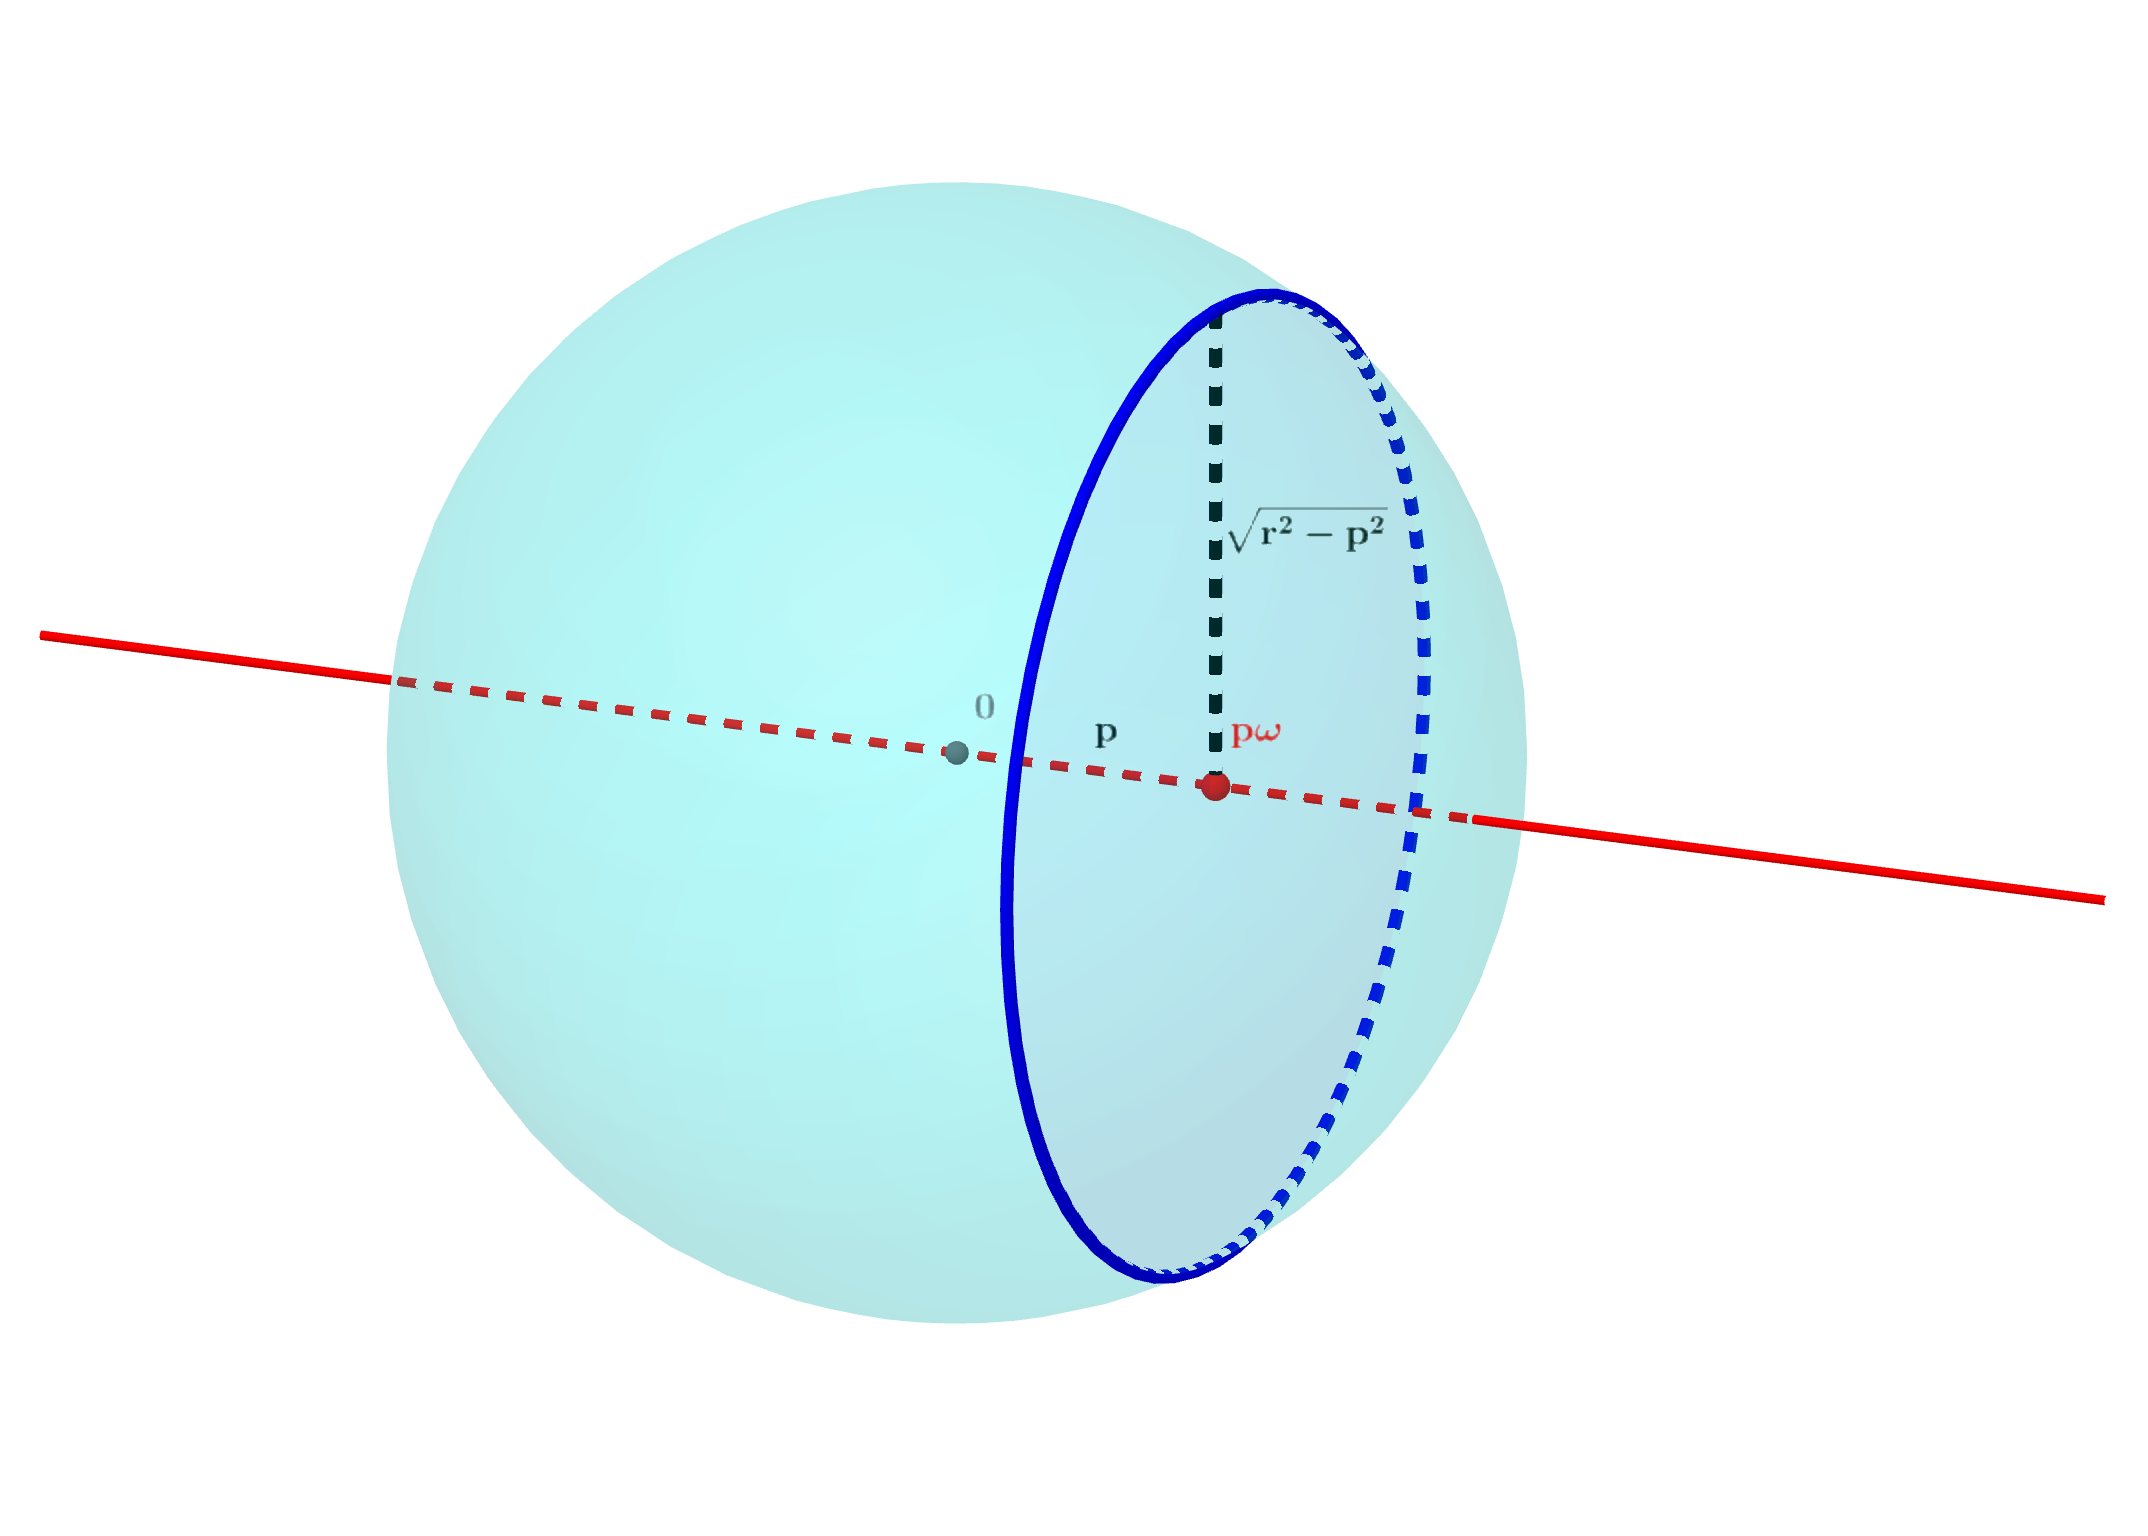
\includegraphics[width=0.7\textwidth]{Images/Ball RT.png}
    \caption{The RT of a ball}\label{fig:RTBall}
  \end{figure}

  We can use this formula to determine the RT of an anulus. Let $A(r_1, r_2) = \{x \in \RR^n: r_1 \leq \|x\| \leq r_2\}$. Then
  \begin{align*}
    R_{A(r_1, r_2)}(\omega, p) 
    &= R_{B(r_2)}(\omega, p) - R_{B(r_1)}(\omega, p) \\
    &= 
    \begin{cases}
      V_{n-1}(\sqrt{r_2^2 - p^2}) - V_{n-1}(\sqrt{r_1^2 - p^2}), & |p| < r_1 \\
      V_{n-1}(\sqrt{r_2^2 - p^2}), & r_1 \leq |p| \leq r_2 \\
      0, & |p| \geq r_2
    \end{cases}
  \end{align*}
\end{myexample}
 


Now consider an example of an unbounded region.

\begin{myexample}
Let $S = \{(x,y) : |y| \leq \frac12\} \subseteq \RR^2$ be a strip centered on the $x$-axis with width $1$. Clearly if $\theta = \pi/2$ or $3\pi/2$ then 
\[
  R_S(\theta, p) = 
  \begin{cases}
      \infty, & |p| \leq \frac12 \\
      0, & |p| > \frac12
  \end{cases}.
\]
Otherwise, 
\[
  R_S(\theta, p) = \sec \theta
\]
Note because $S$ is unbounded, that $R_S$ is not only unbounded, but even divergent in some cases.

\begin{figure}[h]
  \centering
  \begin{tikzpicture}[strip/.style={blue, fill=blue, fill opacity = 0.3},
      angle/.style={red},
      axis/.style={<->,black}]
  %draw axes
  \draw[axis] (-1.5,0) -- (4.5,0) node[anchor=west]{$x$};
  \node at (-.2,-.2) {$0$};
  \draw[axis] (0,-2) -- (0,2) node[anchor=west]{$y$};
  %draw wedge
  \fill[strip] (-1, 1) -- (4,1) -- (4, -1) -- (-1, -1) -- cycle;
  \draw[thick, blue] (-1,1) -- (4,1);
  \draw[thick, blue] (-1,-1) -- (4,-1);
  \node[blue] at (-0.5,0.5) {$S$};
  %draw hyperplane
  \draw[thick, blue, dashed] (1.5,2) -- (3.5,-2);
  \draw[thick, blue] (2,1) -- (3,-1);
  %draw angles
  \def\ra{.5};
  \draw[red] (0,0) -- (2,1);
  \draw[red] (\ra,0) arc (0:26.57:\ra) node[midway, right]{$\theta$};
  \draw[red] (2,1) -- (2,-1);
  \draw[red] (2,-1+\ra/2) -- (2+\ra/2,-1+\ra/2) -- (2+\ra/2,-1);
  \draw[red] (2,1-\ra) arc (270:296.57:\ra);
  % \draw[red] (-1,0) arc (180:135:1)node[midway, left]{$\delta$};
  \end{tikzpicture}
  \caption{RT of a strip}\label{fig:strip}
\end{figure}
% More generally, if $S(\varphi, r_1, r_2) = \{(x,y) : r_1 \leq x \cos \varphi + y \sin \varphi \leq r_2\}$ is a strip then (I'm guessing here)
% \[
%     R_{S(\varphi, r_1, r_2)} =
%     \begin{cases}
%         (r_2 - r_1) \sec (\theta - \varphi), & \theta \neq \varphi \pm \frac\pi2 \\
%         \infty, & \theta = \varphi \pm \frac\pi2 \text{ and } p \in [r_1, r_2] \\
%         0, & \theta = \varphi \pm \frac\pi2 \text{ and } p \not\in [r_1,r_2]
%     \end{cases}
% \]
\end{myexample}

Our main addition to previous work will be the use of a modified RT, the Gaussian Radon transform (GRT). This transform is very similar to the RT, but the inclusion of a Gaussian density $w_{n-1}(x)$ in the integral allows for convergence on a larger class of functions $f$. This includes for example unbounded regions. In a broader context the Gaussian Radon transform also has the advantages of generalizng to infite dimensional Hilbert spaces~\cite{Seng14} (on which the Lebesgue measure is not defined), as well as having a natural probabilistic interpretation.

\begin{definition}
The \textit{Gaussian Radon transform} $GR_f : S^{n-1} \times \RR \rightarrow \RR$ of $f$ is defined similarly to the RT.\@ Given $\omega \in S^{n-1}$ and $-\infty < p < \infty$, the GRT is
\[
  GR_f(\omega, p) = 
  \int\mclimits_{\langle x, \omega \rangle = p} f(x) w_{n-1}(x - p\omega) ~dx.
\]
provided the integral converges. Note the Gaussian density 
\[
  w_{n-1}(x - p\omega) = {(2\pi)}^{-(n-1)/2}e^{-\|x - p\omega\|^2/2}
\] 
is centered on the point of the hyperplane closest to the origin.
\end{definition}

\begin{figure}[h]
    \centering
    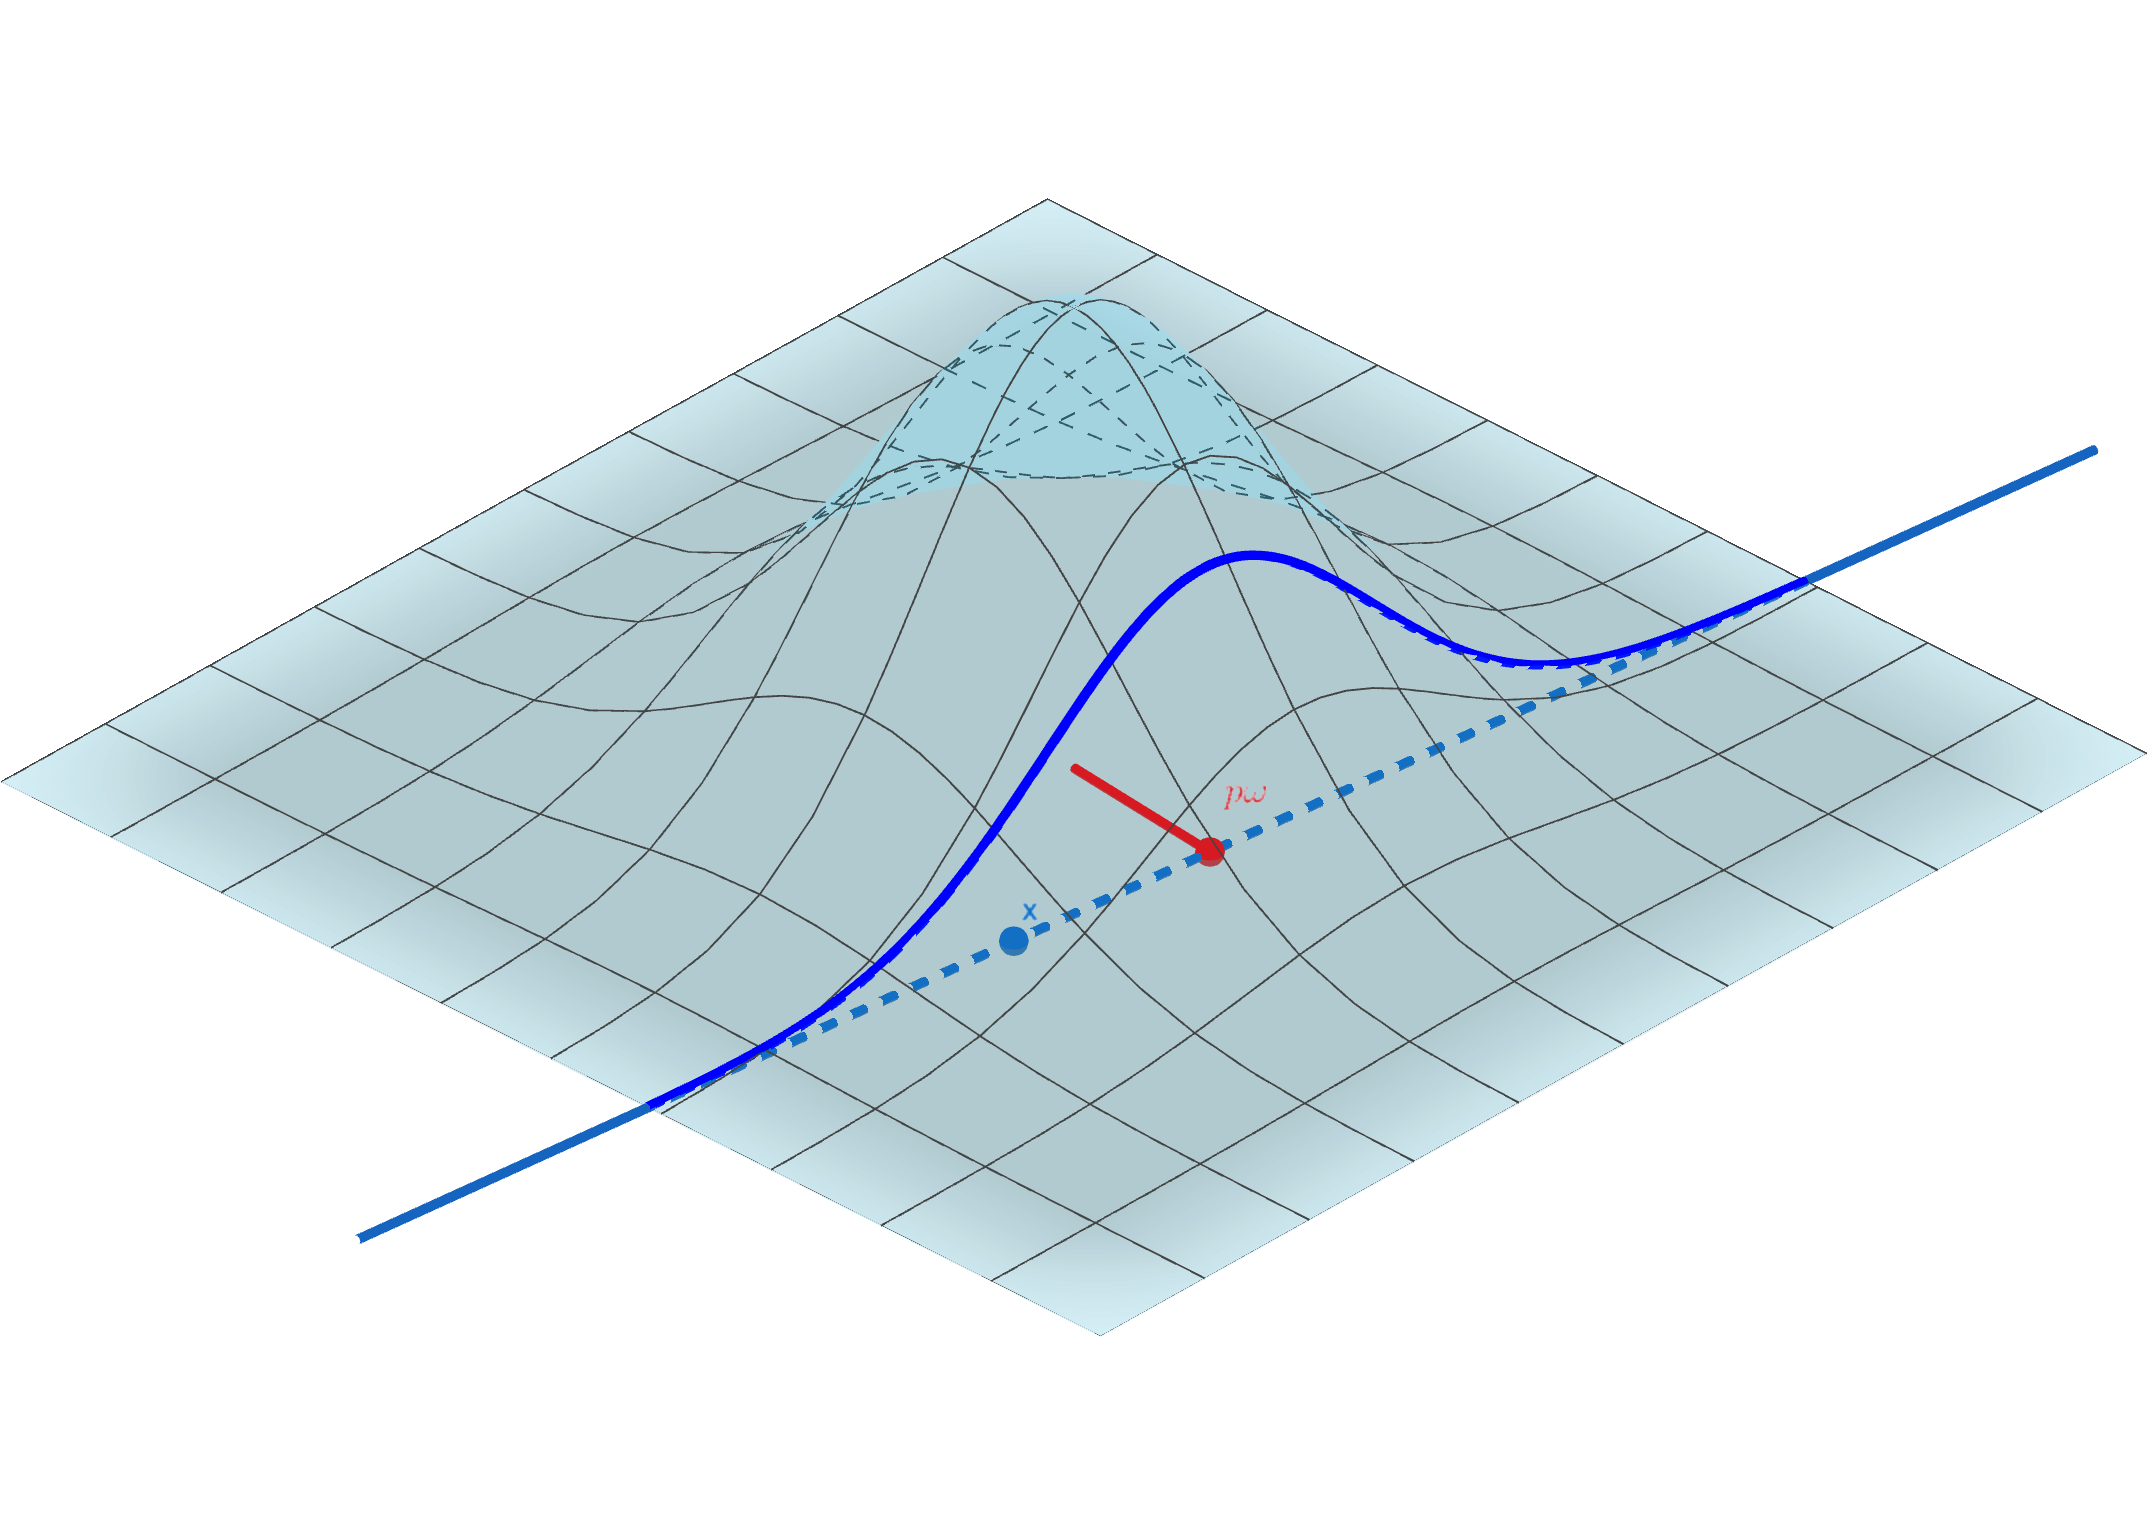
\includegraphics[width=0.7\textwidth]{Images/GRT.png}
    \caption{The GRT}\label{fig:GRT}
\end{figure}

\begin{remark}
  It may be helpful to understand the GRT as a simple modification of the RT with respect to a Gaussian measure on $\RR^n$. From the relation
  \begin{align*}
    \int\mclimits_{\langle x, \omega \rangle = p} f(x) w_n(x) ~dx
    &= \int\mclimits_{\langle x, \omega \rangle = p} f(x) w_{n-1}(x) ~dx~ w(p),
  \end{align*}
  we can express the GRT of $f$ in terms of the $RT$ of the function $g(x) = f(x)w_n(x)$:
  \begin{equation}
    \label{eq:GRTPythag}
    R_g(\omega, p) = GR_f(\omega, p) w(p), \qquad g(x) := f(x)w_n(x).
  \end{equation}
  The relation above provides decent intuition for the GRT, and is also a useful tool proving some basic properties of the transform. Expand on intuition (maybe with example.)
\end{remark}

\begin{myexample}
  If $x(t):\RR^{n-1} \longrightarrow \RR^n$ is a parametrization of $\langle x, \omega\rangle = p$ as described above, then
  \[
    GR_f(\omega, p) = \int_{\RR^{n-1}}f(x(t)) w_{n-1}(t) dt
  \]
  In particular for $f:\RR^2 \rightarrow \RR$
  \[
    GR_f(\omega, p) = \int_{-\infty}^\infty f(t \sin \theta + p \cos \theta, -t \cos \theta + p \sin \theta) w(t)~dt
  \]
  where $\omega = (\cos \theta, \sin \theta)$.
\end{myexample}

\begin{myexample}
  The Gaussian Radon transform is bounded for any measurable region $A \subseteq \RR^n$. Indeed 
  \[
      GR_A(\omega, p) \leq GR_1(\omega, p) = \int_{\RR^{n-1}} w_{n-1}(t)dt w(p) = w(p)
  \]
\end{myexample}

\begin{myexample}
  Consider the Strip $S \subseteq \RR^2$ from [earlier example]. While the RT of $S$ was divergent for $\theta = \pi/2$ or $3\pi/2$, the GRT converges. In particular,
  \[
    GR_S(\theta, p)
    = \begin{cases}
      \frac1{\sqrt{2\pi}}e^{-\frac{p^2}2}, & |p| \leq \frac12 \\
      0, & |p| > \frac12
    \end{cases}
  \]
  This is the density of a ``truncated'' normal distribution on $[-\frac12,\frac12]$. For other angles $GR_S(\theta, p)$ is likewise the density of a truncated normal distribution, this time with arbitrary endpoints $[a, b]$, given by
  \[
    a = ?, \qquad b = a + \sec\theta
  \]
\end{myexample}

Now imagine sweeping a hyperplanar ``slice'' across $\RR^n$. As a function of $p$, $R(\omega, p)$ can be seen as a projection of $f$ onto the linear subspace spanned by $\omega$. It is not surprising that integrating this projection over $-\infty < p < \infty$ we get the same result as the $n$-fold integral of $f$ over $\RR^n$.
\[
    \int_{-\infty}^\infty R(\omega, p) ~dp = \int_{\RR^n} f(x) ~dx
\]
The so called ``slice theorem'' further generalizes this observation:

\begin{proposition}[Slice Theorem]
  % If $f: \RR^n \rightarrow \RR$ and $F: \RR \rightarrow \RR$ are measureable, then
  If $f \in L^1(\RR^n)$ and $F \in L^\infty(\RR)$, then
  % If $f \in C_c(\RR^n)$ and $F \in L^1_{loc}(\RR)$, then
  % \needed{EXTRA CONDITIONS} (i.e. non-negative Fubnini,  Tonelli)
  \begin{align}
    \label{eq:ST}
    \int_{-\infty}^\infty R_f(\omega, p) F(p) dp 
    % &= \int_{-\infty}^\infty \int_{\langle x, \omega \rangle = p} f(x) F(p) ~d\mu(x) ~dp 
    &= \int_{\mathbb{R}^n} f(x) F(\langle x, \omega \rangle) dx,
  \end{align}
  % so long as one of the two is finite.
\end{proposition}

\begin{proof}
  This is a corollary of the Fubini-Tonelli theorem, which guarentees the slice formula as the integrals on eather side converge absolutely. To see this note that there is a rigid transformation (Hilbert space isorphism) taking this to an itterated integral over $\RR^{n-1}$ and $\RR$. Further, $F(\langle x, \omega \rangle) \in L^\infty(\RR^n)$, so the proposition follows by H\"older's inequality
  \[
    \int_{\RR^n} \left|f(x) F(\langle x, \omega \rangle)\right| ~dx \leq \int_{\RR^n}|f(x)| ~dx \|F(\langle x, \omega \rangle)\|_\infty <  \infty
  \] 
  % (under which the Euclidean measures are invariant), the is an integral over $\RR^{n-1}$
  % Fubini's theorem applies since if 
  % Inserting the definition of the RT, the left side is
  % \[
  %   \int_{-\infty}^\infty \int\mclimits_{\langle x, \omega \rangle = p} f(x) ~dx~ F(p) ~dp 
  %   = \int_{-\infty}^\infty \int\mclimits_{\langle x, \omega \rangle = p} f(x) F(\langle x, \omega \rangle) ~dx dp.
  % \]
  % Up to a rigid transformation (under which the Euclidean measures are invariant) this is essentially an itterated integral over $\RR$ and $\RR^{n-1}$. Thus given the integrability requirement, Fubini's theorem applies and the slice theorem is proved.
\end{proof}

\begin{remark}
  % Although we invoke the general Fubini condition here, we note a couple of more convenient sufficient conditions. First, if $f \in L^1(\RR^n)$ and $F \in L^\infty(\RR)$ then,
  The sufficient conditions for the slice theorem above can loosened significantly. We can take for example the straightforward Fubini condition 
  \[
      \int_{\RR^n} |f(x)F(\langle x, \omega \rangle )| < \infty
  \]
  which is necessary \cn, but not convenient. We may also use the condition $f$ has bounded support and $F \in L^1_{loc}(\RR)$.

  The conditions on $f$ and $F$ can be reduced somewhat. In general the convergence of either the left or right side above is sufficient. One 
  % We can specify various conditions for convergence. If $F(p)$ is bounded then $\int |f(x)| dx < \infty$ suffices for convergence. If $f$ is continuous with compact support then $F(p)$ only needs to be integrable.  
\end{remark}

If $F(p) = e^{-ip}$ and $f(x)$ is such that $\int_{-\infty}^\infty R_f(\omega, p) dp < \infty$ then (\ref{eq:ST}) becomes the well known Fourier slice theorem
\[
  \int_{-\infty}^\infty R_f(\omega, p) e^{-ip} ~dp
  = \int_{\mathbb{R}^n} f(x) e^{-i\langle x, \omega\rangle} ~dx,
\]
which is often articulated as saying that the $1$-dimensional Fourier transform of the Radon transform is the $n$-dimenstional Fourier transform of $f$.

An early and natural question in the study of the RT is that of inversion. Radon himself derived the ``Radon inversion formula''~\cite{Rado17}~\cite{Rado86}, which is often proved via the above Fourier slice theorem. The groundbreaking inversion formula is the basis for what, in application, called ``filtered backpropogation''.

If one is interested in inverting the RT then a prerequisite concern is of course: Is the transform injective? The answer clearly depends on what space we draw the function $f$ from. Radon~\cite{Rado17}~\cite{Rado86} provides a set of sufficient regularity conditions such that the RT is invertible. Other similar results followed \cite{????}. On the other hand counterexamples have been constructed by, for example, Lawrence Zalcman~\cite{Zalc82}, of continuous and nontrivial functions for which the RT is identically zero.

By way of the relation (\ref{eq:GRTPythag}) we can prove an analogous slice theorem for the GRT.\@ Mihai and Sengupta prove the general result if real, separable, infinite Hilbert spaces \cn.

\begin{proposition}[Gaussian Slice Theorem] 
  Let $f:\RR^n \rightarrow \RR$ and $F:\RR \rightarrow \RR$ be measurable functions. If $f \in L^1(\RR^n, w_n)$ and $F \in L^\infty(\RR)$ then
  \begin{equation}\label{eq:GST}
    \int_{-\infty}^\infty GR_f(\omega, p)F(p) w(p) ~dp
    = \int_{\mathbb{R}^n}f(x) F(\langle x, \omega\rangle) w_n(x) ~dx. 
  \end{equation}
\end{proposition}

\begin{remark}
  Again the more general Fubini condition
  \[
    \int_{\mathbb{R}^n} |f(x) F(\langle x, \omega\rangle) w_n(x)| dx < \infty
  \]
  may be used. Further, whatever conditions on $f$ and $F$ are sufficient for convergence in (\ref{eq:ST}) are then sufficient conditions to be checked of $f(x)w_n(x)$ and $F(p)w(p)$. I'll need to check these conditions more carefully.
\end{remark}



\begin{proof}
  From (\ref{eq:GRTPythag})
  \[
    \int_{-\infty}^\infty GR_f(\omega, p)F(p) w(p) ~dp 
    = \int_{-\infty}^\infty R_g(\omega, p) F(p) ~dp
  \]
  where $g(x) = f(x)e^{-\|x\|^2/2}$. Note that $\|g\|_1 = \|f\|_{1,w_n} < \infty$ and. Then applying the slice theorem:
  \[
    \int_{-\infty}^\infty R_g(\omega, p) F(p) ~dp 
    = \int_{\RR^n} f(x)F(\langle x, \omega \rangle) w_n(x) ~dx,
  \]
  completing the proof.
\end{proof}

% \begin{remark}
%     For an equivalent 
% \end{remark}

\section{The Radon transform of measures}

% Here we extend the definitions of the RT and GRT to apply to 

Taking from the context of classical moment problems we should define the notion of the Radon transform of a measure $\mu$. Let $\mu$ be a Borel measure on $\RR^n$ with finite moments $c_\alpha$, $\alpha \in \NN_0^n$. The projection $\pi_\omega : \RR^n \rightarrow \RR$ given by
\[
  \pi_\omega(x) = \langle x, \omega \rangle
\] 
is a Borel function, thus we may define the push-forward measure $\mu_\omega = \mu \circ \pi_\omega^{-1}$ which for Borel sets $A \subseteq \RR$ is given by,
\[
  \mu_\omega(A) = \mu(\pi_\omega^{-1}(A)) = \mu(\{x : \langle x, \omega \rangle \in A\}).
\]
We may call $\mu_\omega$ the \emph{marginal projection measure} of $\mu$ with direction vector $\omega$.

Notice that if $\mu$ is absolutely continuous with density representation $\mu = f(x)dx$ then the slice theorem with $F(p)$ the characteristic function of $A$ gives,
\[
  \mu(\pi_\omega^{-1}(A)) = \int\mclimits_{\langle x, \omega \rangle \in A} f(x)dx = \int_A R_f(\omega, p) dp
\]
so that in fact $\mu_\omega$ is absolutely continuous with respect to the Lebesgue measure $dp$ and it's density is precisely the Radon transform $R_f(\omega, p)$. In this sense the marginal projection $\mu_\omega$ is a natural generalization of the RT, so we define

\begin{definition}
  The Radon transform of a Borel measure $\mu$ on $\RR$ is defined as the push-forward measure $\mu_\omega = \mu \circ \pi_\omega^{-1}$ on $\RR$, where $\pi_\omega: \RR^n \rightarrow \RR$ is the projection 
  \[
    \pi_\omega(x) = \langle x, \omega \rangle.
  \]
  We may denote this measure by $R_\mu^\omega = \mu_\omega$.
\end{definition}

\begin{remark}
  It seems that the slice theorem is analogous to — and perhaps generalized by — the change of variables formula for the pushforward measure $R^\omega_\mu$:
  \[
    \int_{-\infty}^\infty F(p) dR^\omega_\mu(p) = \int_{\RR^n} F(\pi_\omega(x)) d\mu
  \]
  where $F:\RR \rightarrow \RR$ is integrable with respect to $dR^\omega_\mu$ if and only if $F\circ\pi_\omega : \RR^n \rightarrow \RR$ is integrable with respct to $\mu$.
\end{remark}
Can we similarly define the GRT of a measure?

\begin{proposition}
  Let $c_\alpha (\omega) = \int_{-\infty}^\infty R_f(\omega, p) p^k dp$ be the projection moments of $f$ at a fixed $\omega$, and $c_\alpha$ the multivariate moments of $f$. Then
  \[
      c_k(\omega) = \sum_{|\alpha| = k}\binom{k}{\alpha} \omega^\alpha c_\alpha
  \]
  where $\binom{k}{\alpha} = \frac{k!}{\alpha_1! \alpha_2! \cdots \alpha_n!}$ are multinomial coefficients.
\end{proposition}

\begin{proof}
  By the slice theorem (\ref{eq:ST}) with $F(p) = p^k$,
  \[
    \int_{-\infty}^\infty R_f(\omega, p) p^k ~dp 
    = \int_{\RR^n} f(x) \langle x, \omega \rangle^k ~dx.
  \]
  Now $\langle x, \omega \rangle^k = {(x_1 \omega_1 + \cdots + x_n \omega_n)}^k$ has the multinomial expansion
  \[
    \langle x, \omega \rangle^k = \sum_{|\alpha| = k}\binom{k}{\alpha} x^\alpha\omega^\alpha.
  \]
  Thus after a bit of rearranging we get
  \begin{align*}
    \int_{\RR^n} f(x) \langle x, \omega \rangle^k ~dx
    &= \int_{\RR^n} f(x) \sum_{|\alpha| = k}\binom{k}{\alpha} x^\alpha \omega^\alpha ~dx \\
    &= \sum_{|\alpha| = k}\binom{k}{\alpha} \omega^\alpha \int_{\RR^n} f(x) x^\alpha ~dx,
  \end{align*}
  where the integrands are precisely the $k$th degree multivariate moments of $f$.
\end{proof}

Similarly, moments of the GRT (Gaussian projection moments) can be expressed in terms of multivariate gaussian moments.

\begin{proposition}
  Let $c_k^G(\omega) = \int_{-\infty}^\infty GR_f(\omega, p) p^k w(p) dp$ be the Gaussian moments of the GRT of $f$ at a fixed $\omega$. Let $c^G_\alpha = \int_{\RR^n} f(x) w_n(x) x^\alpha dx$ be the Gaussian multivariate moments of $f$. Then
  \[
    c^G_k(\omega) = \sum_{|\alpha| = k}\binom{k}{\alpha} \omega^\alpha c^G_\alpha.
  \]
\end{proposition}


\begin{proof}
  The proof follows as it did for the RT.\@ This time we apply the GRT slice theorem (\ref{eq:GST}) with $F(p) = p^k$, 
  \begin{align*}
    \int_{-\infty}^\infty GR_f(\omega, p) p^k w(p) ~dp
    &= \int_{\RR^n} f(x) \langle x, \omega \rangle^k w_n(x) ~dx
  \end{align*}
  Again we use the multinomial expansion of $\langle x, \omega\rangle^n$ and rearange:
  \[
    \int_{\RR^n} f(x) \langle x, \omega \rangle^k w_n(x) ~dx
    = \sum_{|\alpha| = k} \binom{k}{\alpha} \omega^\alpha \int_{\RR^n} f(x) w_n(x)x^\alpha dx. 
  \]
  Thus
  \[
    c^G(\omega) = \sum_{|\alpha| = k} \binom{k}{\alpha} \omega^\alpha c^G_\alpha.
  \]
\end{proof}

\begin{myexample}
  Let $e_1, e_2, \ldots, e_n \in S^{n-1}$ be the the standard basis for $\RR^n$,
  \[
    (1, 0, \ldots, 0),~ (0, 1, \ldots, 0),~ \ldots,~ (0,0, \ldots, 1)
  \]
  Then $\langle x, e_i \rangle = x_i$ is the natural projection of $\RR^n$ onto the $e_i$ axis. The standard projection moments can be calculated as follows
  \begin{align*}
    c_k(e_i) 
    &= \sum_{|\alpha| = k} \binom{k}{\alpha} e_i^\alpha c_\alpha \\
    &= c_{ke_i}
  \end{align*}
  since $e_i^\alpha = 0$ unless $\alpha = ke_i$.
\end{myexample}

The following theorem, due to Petersen \cn, gives a way us to reduce the question of determinacy for multivariate moment problems to the classical case.

\begin{proposition}[Petersen's theorem]
  Let $\mu$ be a Borel measure with finite moments on $\RR^n$, and $e_1, \ldots, e_n$ the standard basis for $\RR^n$. If each $R_\mu^{e_1}, \ldots, R_\mu^{e_n}$ is determinate, then $\mu$ is determinate.
\end{proposition}

\begin{proof}
  An outline of the proof is as follows. Preliminarily, note that the solution set $[\mu]$ of Borel measures with equivalent moments to $\mu$ is convex \cn, and a $\mu$ is an extreme point in $[\mu]$ if and only if polynomials are dense in $L^1(\RR^n, \mu)$ \cn. Thus it suffices to show that polynomials are dense in $L^1(\RR^n, \mu')$ for any $\mu' \in [\mu]$.
  
  The family of products of continuous functions of compact support $f(x) = \prod_{i=1}^n f_i(x_i)$ where each $f_i \in C_c(\RR)$, is dense in $L_1(\mu)$ \cn. Furthermore, since $R_\mu^{e_i}$, $i = 1, \ldots, n$ are determinate, polynomials are dense in each $L^2(\RR, R_\mu^{e_i})$ \cn. Petersen constructs a series of polynomials $P_i : \RR \rightarrow \RR$ such that the polynomial product $P(x) = \prod_{i = 1}^n P_i(x_i)$ arbitrarily close to $f$ in $L^1(\mu)$. Thus polynomials are dense in $L^1(\RR^n, \mu)$ and the moment problem is determinate. \pn 
  
  Note Schm\"udgen proves this via Borel characteristic functions. Not clear what the benefit is.
\end{proof}

\begin{remark}
  Conjecture? We expect this result to hold true for any orthonormal basis, and likely any basis. Will have to check this. Arguable benefit for us is that we in theory can use any $n$ linearly independent projections to reconstruct $\mu$.
\end{remark}

\begin{corollary}
  If $\mu$ is compactly supported Borel measure on $\RR^n$, then the multivariate moment problem is determinate.
\end{corollary}

\begin{proof}
  It suffices to note that the projections $R_\mu^{e_i}$ are compactly supported Borel measures on $\RR$, and thus determinate by \cn.
\end{proof}


We show in section (2.2) that any function $f$ in the weighted space $L^2(\RR, \gamma)$ is determinate (maybe this should be moved to section 1.2). Petersen's theorem allows us to generalize this result to $\RR^n$.

\begin{corollary}
  If $f \in L^2(\RR^n, \gamma^n)$, then $f$ is determinate.
\end{corollary}

\begin{proof}
  % This follows from the product decomposition of the the Gaussian density
  % \[
  %   w_n(x) = \prod_{i = 1}^n w(x_i)
  % \]
  % so that
  % \[
  %   R_f(e_i, p) = \int_{x_i=p} f(x) w_n(x) dx
  % \]
  \pn
\end{proof}

\section{The Radon transform of multivariate Hermite polynomials over general affine subspaces}

% The goal of this section will be to explore the generalizations of the RT and GRT as functions of general affine subspaces. We discuss the analogues of many of the previous results in this context.
We begin this section by proving a formula for the GRT of the multivariate Hermite polynomials defined in the previous section. Recall that for $\alpha \in \NN_0^n$ the polynomials $H_\alpha(x)$ can be defined by the generating function
\[
  e^{\langle x, y\rangle - \frac{\|y\|^2}2} = \sum_{\alpha \in \NN_0^n} \frac{H_\alpha(x)}{\alpha!} y^\alpha
\]
where $\alpha! = \alpha_1! \cdots \alpha_n!$. These are related to the classical Hermite polynomials by
\[
  H_\alpha(x) = \prod_{i=1}^n H_{\alpha_i}(x_i)
\]
where, for $k \in \NN_0^\infty$, the classical polynomials $H_{k}(p)$ can be defined by
\[
  e^{pt - \frac{t^2}2} = \sum_{k = 0}^\infty \frac{H_k(p)}{k!}t^k.
\]

\begin{proposition} \label{prop:GRTHermite}
  Let $\omega \in S^{n-1}$ and $p \in \RR$ be fixed. If $|\alpha| = k$, then the GRT of the multivariate Hermite polynomial $H_\alpha$ is
  \[
    GR_{H_\alpha}(\omega, p) = H_k(p)\omega^\alpha
  \]
\end{proposition}

\begin{proof}
  Recall that the generating function $\phi(x) = e^{\langle x, y\rangle - \frac{\|y\|^2}2}$ converges absolutely for all $x,y \in \RR^n$. Consider the GRT of $\phi$,
  \begin{align*}
    GR_{\phi}(\omega, p) 
      &= \int\mclimits_{\langle x, \omega \rangle = p} \phi(x) w_{n-1}(x - p\omega)~dx.
    % \\&= \int\mclimits_{\langle x, \omega \rangle = 0} \phi(x + p\omega) w_{n-1}(x)~dx
  \end{align*}
  Immediately we can expand $\phi(x)$, interchanging integral and series, to see
  \begin{equation} \label{eq:GRTPhiExpansion1}
    \begin{split}
      GR_{\phi}(\omega, p)
        &= \sum_{\alpha \in \NN_0^n} \frac1{\alpha!} y^\alpha \int\mclimits_{\langle x, \omega\rangle = p} H_\alpha(x) w_{n-1}(x - p\omega)~dx
      \\&= \sum_{\alpha \in \NN_0^n} \frac{GR_{H_\alpha}(\omega, p)}{\alpha!} y^\alpha.
    \end{split}
  \end{equation}
  On the other hand, we will be able to show that
  \begin{equation} \label{eq:GRTPhiExpansion2}
    GR_{\phi}(\omega, p) 
    = \sum_{k = 0}^\infty \sum_{|\alpha| = k} \frac{H_k(p)\omega^\alpha}{\alpha!} y^\alpha.
  \end{equation}
  Thus, being careful to note that the series (\ref{eq:GRTPhiExpansion1}) and (\ref{eq:GRTPhiExpansion2}) converge absolutely, we can compare coefficients for the desired formula. In order to derive the second expansion we begin by translating our integral onto the linear subspace $\langle x, \omega\rangle = 0$, via the change of variables $x \mapsto x + p\omega$:
  \begin{equation}\label{eq:GRTPhiExpansion21}
    \begin{split}
      GR_{\phi}(\omega, p) 
        &= \int\mclimits_{\langle x, \omega\rangle = 0} \phi(x + p\omega) w_{n-1}(x) ~dx 
      \\&= \int\mclimits_{\langle x, \omega\rangle = 0} e^{\langle x + p\omega, y \rangle - \frac{\|y\|^2}2}(2\pi)^{-\frac{n-1}2}e^{-\frac{\|x\|^2}2} ~dx
      \\&= e^{p \langle \omega, y\rangle - \frac{\|y\|^2}2} \int\mclimits_{\langle x, \omega\rangle = 0}e^{\langle x, y\rangle - \frac{\|x\|^2}2} (2\pi)^{-\frac{n-1}2} ~dx
    \end{split}
  \end{equation}
  Now in order to compute the right side integral we consider the orthogonal decomposition $y = y_\omega + y_{\omega^\perp}$, where
  \[
    y_\omega = \langle y, \omega \rangle \omega \qquad y_{\omega^\perp} = y - y_\omega.
  \]
  We make two observations about this decomposition of $y$: First, 
  \begin{equation}\label{eq:GRTPhiExpansion22}
    \|y\|^2 
      = \|y_\omega\|^2 + \|y_{\omega^\perp}\|^2 
      = \langle y, \omega\rangle^2 + \|y_{\omega^\perp}\|^2
  \end{equation}
  and second, for $x$ in the linear subspace $\langle x, \omega\rangle = 0$ we have
  \[
    \langle x, y \rangle
      = \langle x, \omega \rangle \langle y, \omega \rangle + \langle x, y_{\omega^\perp} \rangle 
      = \langle x, y_{\omega^\perp} \rangle.
  \]
  This second observation allows us to solve the integral at the end of (\ref{eq:GRTPhiExpansion21}). By completing the square $\|x - y_{\omega^\perp}\| = \|y_{\omega^\perp}\|^2 - 2\langle x, y_{\omega^\perp} \rangle + \|x\|^2$, we have
  \begin{align*}
    \int\mclimits_{\langle x, \omega\rangle = 0}e^{\langle x, y\rangle - \frac{\|x\|^2}2} (2\pi)^{-\frac{n-1}2} ~dx
      &= e^{-\frac{\|y_{\omega^\perp}\|^2}2} \int\mclimits_{\langle x, \omega\rangle = 0}e^{-\frac{\|y_{\omega^\perp}\|^2}2 + \langle x, y_{\omega^\perp}\rangle - \frac{\|x\|^2}2} (2\pi)^{-\frac{n-1}2} ~dx
    \\&= e^{-\frac{\|y_{\omega^\perp}\|^2}2} \int\mclimits_{\langle x, \omega\rangle = 0}e^{-\frac{\|x - y_{\omega^\perp}\|}2} (2\pi)^{-\frac{n-1}2} ~dx
    % \\&= e^{-\frac{\|p_{\omega^\perp}\|^2}2}
  \end{align*}
  which is just $e^{-\frac{\|p_{\omega^\perp}\|^2}2}$. It was important here to invoke the orthogonal projection $y_{\omega^\perp}$ so that the integrand becomes the translation of a standard Gaussian function on the hyperplane $\langle x, \omega \rangle = 0$. Now returning to (\ref{eq:GRTPhiExpansion21}), we have
  \begin{align*}
    GR_{\phi}(\omega, p) 
      &= e^{p \langle \omega, y\rangle - \frac{\|y\|^2}2-\frac{\|y_{\omega^\perp}\|^2}2}
    \\
      &= e^{p \langle \omega, y\rangle - \frac{\langle y, \omega\rangle^2}2}
  \end{align*}
  where we used (\ref{eq:GRTPhiExpansion22}). This looks like the generating function for the univariate Hermite polynomials $H_k(p)$ with $t = \langle \omega, y \rangle$, so we expand
  \begin{align*}
    GR_{\phi}(\omega, p) 
      &= \sum_{k = 0}^\infty \frac{H_k(p)}{k!} \langle \omega, y\rangle^k.
  \end{align*}
  Finally we apply the multinomial expansion of $\langle \omega, y\rangle^k$, recalling the multinomial coefficients $\binom{k}{\alpha} = \frac{k!}{\alpha!}$. Therefore
  \begin{align*}
    GR_{\phi}(\omega, p)
      &= \sum_{k = 0}^\infty \sum_{|\alpha| = k} \frac{H_k(p)}{k!} \binom{k}\alpha y^\alpha\omega^\alpha
    \\
      &= \sum_{k = 0}^\infty \sum_{|\alpha| = k} \frac{H_k(p)\omega^\alpha}{\alpha!} y^\alpha
  \end{align*}
  as needed.
\end{proof}

\begin{remark}
  The proof above was written by Dr. Sengupta.
\end{remark}

In section 1.4 we defined the RT and GRT as the integrals of a function $f: \RR^n \rightarrow \RR$ over $n-1$ dimensional hyperplanes, the standard definitions. But there are many examples of geometric integral transforms, closely related to the hyperplane RT, which can be thought of as ``generalized Radon transforms''. In fact, the ``Funk transform'', which relates a function on the sphere $S^{3}$ to its integrals over great circles, was first introduced by Paul Funk in 1911, half a decade before Radon introduced the hyperplane RT. In the remainder of this chapter we discuss the notion of the RT and GRT on general $d$-dimensional affine subspaces of $\RR^n$, where $d = 0, \ldots, n$. For context, note that when $d = 1$, this is the so called ``X-ray transform'' which gets it's name from the direct application to radiology.

Let $\Lambda_0$ be a $d$-dimensional linear subspace of $\RR^n$, and $p \in \RR^n$. Then the translation of $\Lambda_0$ by $p$
\[
  \Lambda = p + \Lambda_0
\]
is called an \emph{affine subspace} of $\RR^n$. The representation above is clearly not unique since adding any member of $\Lambda_0$ to $p$ does not change $\Lambda$. However, given an affine subspace $\Lambda$ we have a canonical choice for $p$ as the closest point in $\Lambda$ to the origin. This point exists and is unique since $\Lambda$ is closed and convex. Furthermore the point $p$ defined in this way must be orthogonal to any vector in the linear subspace $\Lambda_0$. That is, $p \in \Lambda_0^\perp$, where $\Lambda_0^\perp$ is the linear subspace
\[
  \Lambda_0^\perp = \{x \in \RR^n : \langle x, y \rangle = 0 \text{ for all } y \in \Lambda\}
\]
also known as the \emph{orthogonal complement} of $\Lambda_0$. Thus we rephrase our definition as follows:

\begin{definition}
  An \emph{affine subspace} $\Lambda$ of dimension $d$ in $\RR^n$ is defined uniquely by
  \[
    \Lambda = p + \Lambda_0
  \]
  where $\Lambda_0$ is a linear subspace of dimension $d$ and $p \in \Lambda_0^\perp$. Sometimes we call $\Lambda$ a ``$d$-plane''.
\end{definition}

\begin{remark}
  Note that the hyperplanes in the original definition of the RT are $(n-1)$-planes, and the lines in the ``X-ray transform'' are $1$-planes.
\end{remark}

Recall that if $\Lambda_0$ is a fixed linear subspace of dimension $d$, the orthogonal complements $\Lambda_0^\perp$ is a linear subspace of dimension $n - d$. For any $x \in \RR^n$ there is a unique orthogonal decomposition $x = x_{\Lambda_0} + x_{\Lambda_0^\perp}$ where $x_{\Lambda_0} \in \Lambda_0$ and $x_{\Lambda_0^\perp} \in \Lambda_0^\perp$. This idea can be summarized by the expression
\[
  \RR^n = \Lambda_0 \oplus \Lambda_0^\perp.
\]

Sometimes it is convenient to have an explicit coordinate system on an affine subspace. If $u^{(1)}, \ldots, u^{(d)}$ is a orthonormal basis for $\Lambda_0$ then there is an isometric embedding of $\RR^d$ into $\RR^n$ with image $\Lambda$ given by $x(t) : \RR^d \rightarrow \Lambda$ where
\[
  x(t) = p + t_1u^{(1)} + \cdots + t_d u^{(d)}, \qquad t \in \RR^d.
\]
By this embedding can define the Euclidean measure $dx$ on $\Lambda$ as the push-forward of the Lebesgue measure on $\RR^n$, and the standard Gaussian measure on $\Lambda$ as the push-forward of $\gamma^n$. Note the $x(t)$ is defined in such a way that $x(0) = p$ which is essential when defining the Gaussian measure on $\Lambda$.

Other times we prefer not to invoke a basis-dependent isometry, and while $x(t)$ clearly depends on the choice of $u^{1}, \ldots, u^{(d)}$, we should note that the Euclidean and Gaussian measures on $\Lambda$ are independent of basis \pn.


Now we can define the natural analogue of the RT for affine subspaces, which is sometimes called the \emph{d-plane transform}.

\begin{definition}
  Let $f:\RR^n \rightarrow \RR$. For any affine subspace $\Lambda = p + \Lambda_0$, we define the \emph{Radon Transform of $f$ on $\Lambda$} by
  \[
    R_f(\Lambda) = \int_{\Lambda} f(x)~dx
  \]
  and the \emph{Gaussian Radon Transform of $f$ on $\Lambda$} by 
  \[
    GR_f(\Lambda) = \int_{\Lambda} f(x) w_d(x - p) ~dx
  \]
  where $d$ is the dimension of $\Lambda_0$.
\end{definition}
\begin{remark}
  Explicitly, if $x(t): \RR^d \rightarrow \Lambda$ is an Euclidean isometry then 
  \[
    R_f(\Lambda) = \int_{\RR^d} f(x(t))~dt
  \]
  If furthermore $x(0) = p$ then
  \[
    GR_f(\Lambda) = \int_{\RR^d} f(x(t))w(t)~dt
  \]
  However keep in mind that these definitions are independent of the particular isometry \pn.
\end{remark}

% To illustrate the calculation of a GRT with an explicit isometry, let
% \[
%   f(x) = e^{\langle x, y\rangle}
% \]
% for some $y \in \RR$. Suppose $\Lambda = p + \Lambda_0$ is a $d$-dimensional affine subspace and $x(t) : \RR^d \rightarrow \Lambda$ is the isometry given by
% \[
%   x(t) = p + \sum_{i = 1}^d t_iu^{(i)}
% \]
% where $u^{(1)}, \ldots, u^{(d)}$ is an orthonormal basis for $\Lambda_0$. Furthermore let $y = y_{\Lambda_0} + y_{\Lambda_0^\perp}$ and note that $\langle x, y \rangle = \langle x, y_{\Lambda_0}\rangle$ for $x \in \Lambda_0$. Then
% \begin{align*}
%   GR_f(\Lambda) 
%     &= \int_{\RR^d} e^{\langle x(t), y \rangle} (2\pi)^{-\frac{d}2} e^{-\frac{\|t\|^2}2}~dt
%   \\
%     &= e^{\langle p, y \rangle} \int_{\RR^d} e^{\sum_{i = 1}^d t_i\langle u^{(i)}, y_{\Lambda_0}\rangle - \frac{\|t\|^2}2} (2\pi)^{-\frac{d}2} ~dt
%   \\
%     &= e^{\langle p, y \rangle} \int_{-\infty}^\infty \prod_{i=1}^d e^{t_i\langle u^{(i)}, y_{\Lambda_0}\rangle - \frac{t_i^2}2} (2\pi)^{-\frac12} dt_i
% \end{align*}
% Now notice in each exponential in the product we can complete the square $\|t_iu^{(i)} - y_{\Lambda_0}\|^2 = \|y_{\Lambda_0}\|^2 - 2t_i\langle u^{(i)}, y_{\Lambda_0}\rangle + t_i^2$, that is
% \[
%   e^{t_i\langle u^{(i)}, y_{\Lambda_0}\rangle - \frac{t_i^2}2}
%     = e^{\frac12\|y_{\Lambda_0^\perp}\|}e^{-\frac12\|t_iu^{(i)} - y_{\Lambda_0}\|^2}
% \]
% for $i = 1, \ldots, d$. The right hand integral is a Gaussian integral equal to $1$. Thus
% \[
%   GR_f(\Lambda) = e^{\langle p, y \rangle} \prod_{i=1}^d 
% \]

% Let's see if we can derive a formula for the GRT of the multivariate Hermite polynomials on a general affine plane.

% Following the proof for the hyperplane GRT, we begin again with the transform of the generating function
% \[
%   GR_\phi(\Lambda)
%     = e^{p\langle \omega, y\rangle - \frac{\|y\|^2}2} \int_{\Lambda_0} e^{\langle x, y\rangle - \frac{\|x\|^2}2} (2\pi)^{-\frac d2}~dx
% \]
% which can be immediately expanded as 
% \[
%   GR_\phi(\Lambda) = \sum_{\alpha!}\frac{GR_{H_\alpha}(\Lambda)}{\alpha!}y^\alpha
% \]
% As before, we decompose $y = y_{\Lambda_0} + y_{\Lambda_0^\perp}$, substitute $y_{\Lambda_0}$ for $y$ and complete the square so that the right hand integral is $e^{\frac{\|y_{\Lambda_0}\|^2}2}$.
% \[
%   GR_\phi(\Lambda) 
%     = e^{p\langle \omega, y\rangle - \frac{\|y\|^2}2 + \frac{\|P_{\Lambda_0} y\|}2}
% \]
% Now we have $\|y\|^2 = \|y_{\Lambda_0}\|^2 + \|y_{\Lambda_0^\perp}\|^2$, so
% \[
%   GR_\phi(\Lambda) 
%     = e^{p\langle \omega, y\rangle - \frac{\|y_{\Lambda_0^\perp}\|^2}2}
% \]
% Here we encounter a problem we didn't see in the hyperplane case: 
% In the hyperplane case $\dim(\Lambda_0^\perp) = 1$ so that $y_{\Lambda_0^\perp}$ was necessarily in the span of $\omega$. But for lower dimensional affine subspaces there is no immediate relation between $y_{\Lambda_0^\perp}$ and $\langle \omega, y\rangle$. 

% If we suppose for the moment that $y \in \Lambda_0^\perp$. Then we do have 
% \[
%   GR_\phi(\Lambda) 
%     = e^{p\langle \omega, y\rangle - \frac{\|y\|^2}2}
%     = \sum_{\alpha \in \NN_0^n} \frac{H_{\alpha}(p\omega)}{\alpha!}y^\alpha
% \]
% so can we conclude $GR_{H_\alpha}(\Lambda) = H_\alpha(p\omega)$? That doesn't feel right.

% If we further suppose that $y$ is in the span of $\omega$ then we find
% \[
%   something else
% \]
% via Ambar

% What if we just assume $\|y_{\Lambda_0^\perp}\|^2 = \langle\omega, y\rangle^2$? This is true essentially if $y \in \omega\RR + \Lambda_0$. In this case we have what we want,
% \[
%   \sum_{\alpha \in \NN_0^n} \frac{GR_{H_\alpha}(\Lambda)}{\alpha!} y^\alpha = \sum_{k=0}^\infty \sum_{|\alpha| = k} \frac{H_k(p)\omega^\alpha}{\alpha!} y^\alpha
% \]
% It doesn't seem like it should be enough for this to hold on a $d+1$ subspace, to conclude that we can compare coefficients. 
% Now if $\omega$ and $P_{\Lambda_0^\perp} y$ are potentially linearly independent, where can we go from here?

% Recall $\omega$ was chosen from $S^{n-1} \cap \Lambda_0^\perp$ and $y \in \RR^n$ is arbitrary, while $P_{\Lambda_0^\perp} y$ is in $\Lambda_0^\perp$. Suppose that $v^{(1)}, \ldots, v^{(n - d)}$ is an orthonormal basis for $\Lambda_0^\perp$. We can write
% \[
%   \omega = \sum_{i = 1}^{n-d} r_i v^{(i)}, \qquad y = \sum_{i = 1}^{n-d} s_i v^{(i)}
% \]
% for some $r,s \in \RR^{n-d}$.

% Is it true that $\langle \omega, y \rangle = \langle \omega, P_{\lambda_0^\perp} y\rangle$? Well, yes: $y = P_{\Lambda_0} y + P_{\Lambda_0^\perp} y$, so
% \[
%   \langle \omega, y \rangle = \langle \omega, P_{\Lambda_0} y \rangle + \langle \omega, P_{\Lambda_0^\perp} y \rangle
% \]
% and $\langle \omega, P_{\Lambda_0} y \rangle = 0$. Then 
% \begin{align*}
%   e^{p\langle \omega, y\rangle - \frac{\|P_{\Lambda_0^\perp} y\|^2}2}
%     &= e^{p\langle \omega, P_{\Lambda_0^\perp} y \rangle - \frac{\|P_{\Lambda_0^\perp} y\|^2}2}
%   \\&= \sum_{\alpha \in \NN_0^n} \frac{H_\alpha(p\omega)}{\alpha!} (P_{\Lambda_0^\perp} y)^\alpha
%   \\&=? \sum_{\alpha \in \NN_0^{n-d}} \frac{H_\alpha(p\omega)}{\alpha!} (P_{\Lambda_0^\perp} y)^\alpha
% \end{align*}
% We still cannot compare coefficients with
% \[
%   \int_\Lambda e^{\langle x, y\rangle - \frac{\|y\|^2}2} w_{d}(x -p\omega)~dx
%     = \sum_{\alpha \in \NN_0^n} \frac{GR_{H_\alpha}(\omega, p)}{\alpha!} y^\alpha
% \]



  % \chapter{Long Title}{Short Title}
% The Long Title will appear on the first page of the chapter.
% The Short Title will appear in the table of contents.
% If the Long Title isn't all that long, you can just call
% \chapter{Long Title}{} and the same title will appear in
% both places.


\chapter{Convergence of Pad\'e approximants}{}

Here we, hear ye, discuss the convergence of rational approximations to the Stieltjes transform. Namely, the Pad\'e approximants to the moment series are defined and convergence to the Stieltjes transform is proved under certain restrictions.

\section{The Markov and Hamburger transforms}

Let $\mu$ be a Borel measure with finite moments $c_k = \int_{-\infty}^\infty p^k d\mu$. 

\begin{definition}
  The complex function $g$ defined by
  \[
    g(z) = \int_{-\infty}^\infty\frac{d\mu}{1+zp}
  \]
  is called the Markov (Hamburger resp.) transform of $\mu$ when $\mu$ has bounded (unbounded resp.) support.
\end{definition}

It is worth noting at the outset that $g(z)$ is defined at least for non-real $z$. To see this we note that if $\im z \neq 0$,
\begin{align*}
  \frac1{|1 + zp|} 
  &= \frac{|1/z|}{|\frac1z + p|} \\
  &\leq \frac{|1/z|}{|\im \frac1z|} \\
  &= \frac{|\overline{z}|/|z|^2}{|\im \overline{z}|/|z|^2} \\
  &= \frac{|z|}{|\im z|}
\end{align*}
which gives the bound
\begin{equation}
  |g(z)| 
  \leq \int_{-\infty}^\infty \frac{|z|}{|\im z|} d\mu(p) 
  = \frac{|z|}{|\im z|}c_0
\end{equation}

Since the integrand has a singularity only when $p = -1/z$ a Markov transform must converge in some neighborhood of zero. This cannot be said in general for a Hamburger transform. 

\begin{remark}
  The bound above has a useful geometric interpretation. For starters we note that,
  \[
    \frac{|\im z|}{|z|} = |\sin(\arg z)|,
  \]
  which can be seen by considering the right triangle formed by the points $0$, $z$, and $\re z$. Thus this bound essentially depends on the angle of separation between $z$ and the real line. 
\end{remark}

\begin{proposition}
  The function $g(z)$ is analytic on the upper and lower half planes $\im z \neq 0$.
\end{proposition}

\begin{proof}
  Let $z, w$ be complex numbers with non-zero imaginary part. We have
  \begin{align*}
    g(w) - g(z)
    &= \int_{-\infty}^\infty \frac{1}{1 + wp} - \frac1{1 + zp}d\mu(p) \\
    &= \int_{-\infty}^\infty \frac{(1 + zp) - (1 + wp)}{(1 + wp)(1 + zp)}d\mu(p) \\
    &= (w - z) \int_{-\infty}^\infty \frac{-p}{(1 + wp)(1 + zp)}d\mu(p).
  \end{align*}
  Thus it seems
  \[
    \lim_{w \rightarrow z} \frac{g(w) - g(z)}{w - z} = \int_{-\infty}^\infty \frac{-p}{(1+zp)^2}d\mu(p).
  \]
  To be precise we may justify the interchange of limit and integral here by dominated convergence. Recall that it suffices to find an integrable function $h : \RR \to \CC$ such that, for any $w$ in a neighborhood of $z$,
  \[
    \left|\frac{-p}{(1 + wp)(1 + zp)}\right| \leq h(p) \qquad \hbox{for all $p \in \RR$}.
  \]
  It should be noted that our particular dominating function $h(p)$ is somewhat arbitrary, and not a sharp bound. By the previously discussed bound we have,
  \[
    \left|\frac{-p}{(1 + wp)(1 + zp)}\right| \leq |p|\frac{|wz|}{|\im w ~\im z|}.
  \]
  Furthermore $|w|/|\im w|$ is clearly continuous on the half planes, so in some neighborhood of 
  \[
    |p|\frac{|wz|}{|\im w ~\im z|} \leq |p|\left(\frac{|z|^2}{|\im z|^2} + \epsilon\right)
  \]
  for an arbitrary $\epsilon > 0$. Finally, we note that the right hand dominating function above is integrable since $\mu$ has finite moments: 
  \[
    \int_{-\infty}^\infty |p| d\mu \leq \int_{-\infty}^\infty \frac12(p^2 + 1) ~d\mu = c_2 + c_0
  \]
\end{proof}

\begin{remark}
  Since $\mu$ is a real measure, $g(z)$ commutes with conjugation,
  \[
    g(\bar z) = \int_\infty^\infty\frac{d\mu}{1+\bar zp} = \overline{\int_\infty^\infty\frac{d\mu}{1+zp}} = \overline{g(z)}.
  \]
  For this reason, although $g(z)$ is defined for all non-real $z$, we will only concern ourselves with its values on the upper half plane $\im z > 0$ going forward. In chapter 3 we should restrict our sample points to the upper half plane, since samples in the lower half may be redundant.
\end{remark}


When $z$ is a real number $g(z)$ may not converge. In particular $g(z)$ does not converge when $z = -1/p$ for some $p$ in the support of $\mu$ \pn.  Thus if $\mu$ has bounded support $g$ converges in a neighborhood of $0$. On the other hand if $\mu$ has unbounded support $g(0)$ is not defined. However — as we will see — even in the Hamburger transform case, a formal series expansion at $z = 0$ holds valuable information. The results of this section are described in detail in section 5.6 of (Baker) \cn

By a geometric series expansion,
\[
  \frac1{1 + zp} = \sum_{k = 0}^\infty {(-z)}^k p^k 
\]
when $|zp| < 1$. This suggests the connection between $g(z)$ and the moment sequence ${(c_k)}_{k \in \NN_0}$. Indeed, at least formally,
\begin{align*}
  \int_\infty^\infty\frac{d\mu}{1+zp}
  &= \int_\infty^\infty \sum_{k = 0}^\infty {(-z)}^k p^k ~d\mu \\
  &= \sum_{k = 0}^\infty {(-z)}^k \int_\infty^\infty p^k ~d\mu \\
  &= \sum_{k = 0}^\infty c_k{(-z)}^k.
\end{align*}
In the Markov case we have a positive radius of convergence. But even in the Hamburger case, there is a sense in which this assymptotic expansion holds ``non-tangentially''.

Non-tangential convergence at $z = 0$ is, as the name implies, convergence along curves not tangent to the real line at $0$. More precisely, one defines a ``wedge domain''
\[
  \Gamma_\delta = \{\delta \leq \arg z \leq \pi - \delta\}
\]
\begin{figure}
  \centering
  \begin{tikzpicture}[wedge/.style={blue, fill=blue, fill opacity = 0.3}, angle/.style={red}, axis/.style={<->,black}]
    %draw axes
    \draw[axis] (-3,0) -- (3,0) node[anchor=west]{$\text{Re} z$};
    \node at (-.2,-.2) {$0$};
    \draw[axis] (0,-1) -- (0,3) node[anchor=west]{$\text{Im} z$};
    %draw wedge
    \fill[wedge] (0, 0) -- (-2.5, 2.5) -- (2.5,2.5) -- cycle;
    \draw[thick, blue] (-2.5, 2.5) -- (0,0) -- (2.5,2.5);
    \node[left, blue] at (0,1.5) {$\Gamma_\delta$};
    %draw angle
    \def\ra{.07};
    \draw[red] (1,0) arc (0:45:1) node[midway, right]{$\delta$};
    \draw[red] (-1,0) arc (180:135:1)node[midway, left]{$\delta$};
  \end{tikzpicture}
  \caption{A wedge domain}\label{fig:wedge}
\end{figure}
in which curves approach $0$ with an angle at least $\delta$ from the real line.

\begin{definition} (Non-tangential convergence and assymptotic expansion)
  We say $h(z) \rightarrow 0$ non-tangentially as $z \rightarrow 0$ if, for any $\delta > 0$, the limit 
  \[
    \lim_{z \rightarrow 0} h(z) = 0
  \]
  holds for $z$ in the $\Gamma_\delta$. If a formal power series $\sum_{k=0}^\infty a_k z^k$ and a function $g(z)$ are such that for all $n\in \NN_0$,
  \[
    g(z) = \sum_{k = 0}^{n-1} c_k{(-z)}^k + z^n h_n(z)
  \]
  where the trailing terms $h_n(z)$ converge to $0$ non-tangentially as $z \rightarrow 0$, we say that $\sum_{k=0}^\infty a_k z^k$ is an assymptotic expansion of $g(z)$. We use the notation
  \[
    g(z) \simeq \sum_{k=0}^\infty a_k z^k
  \]
  for assymptotic expansions.
    % If for any $\delta > 0$ the limit $g(z) \rightarrow L$ holds 
\end{definition}

While $g(z)$ does not generally converge at $z = 0$, in a non-tangential sense the afformentioned assymptotic expansion holds:
\begin{proposition}
  \begin{enumerate}
    \item If $\mu$ has bounded support
    \[
      g(z) = \sum_{k = 0}^\infty c_k{(-z)}^k
    \]
    in a neighboorhood of $z=0$.
    \item For all $n \in \NN_0$
    \begin{equation}
      g(z) = \sum_{k = 0}^{n-1} c_k{(-z)}^k + z^n h_n(z) \label{assexp}
    \end{equation}
    where $h_n$ is such that $\lim_{z \rightarrow 0} h_n(z) = 0$ non-tangentially.
  \end{enumerate}
\end{proposition}

\begin{proof}
  We first note that 
  \[
    \sum_{k=0}^{n} c_k {(-z)}^k 
    = \sum_{k=0}^{n} \int_{-\infty}^\infty {(-zp)}^k d\mu
    % = \int_{-\infty}^\infty \sum_{k=0}^{n} (-zx)^k d\mu
    = \int_{-\infty}^\infty \frac{1 - {(-zp)}^{n+1}}{1 + zp} d\mu
  \]
  and so
  \begin{align*}
    h_n(z) = \frac1{z^n}\left\{g(z) - \sum_{k=0}^{n} c_k {(-z)}^k\right\}
    &= \int_{-\infty}^\infty \frac{zp^{n+1}}{1 + zp}d\mu.
  \end{align*}
  It remains to determine if and in what sense this trailing term $h_n(z)$ vanishes at the origin. 

  As expected in the case when $\mu$ has bounded support, $h_n(z)$ exists in a neighborhood of $0$ and vanishes as $z \rightarrow 0$ in this neighboorhood. Thus the assymptotic expansion~\ref{assexp} is the Taylor expansion: The Markov transform is analytic at the origin.

  When $\mu$ has unbounded support and $h_n(z)$ may not be well defined on the real line, so we must weaken our result to non-tangential convergence. If $z \in \Gamma_\delta$ then we have the following inequalities for any $p \in \RR$,
  \[
    |p - z| \geq |p| \sin \delta 
    \quad\text{and} \quad
    |p - z| \geq |p| \sin \delta.
  \]
  We will show that
  \[
    \lim_{z \rightarrow 0} h_{2n}(z) = 0, \quad z \in \Gamma_\delta
  \]
  from which the corresponding limit for odd orders will immediately follow from the relation
  \[
    h_{2n-1}(z)
    = zh_{2n}(z) + c_{2n}z^{2n}.
  \] 
  Here for the sake of convenience we define $w = -\frac1z$, following a more classical approach. Note that $|w| = \frac1{|z|}$ and if $z$ is in the wedge $\Gamma_\delta$ then so is $w$. Now 
  \begin{align*}
    |h_{2n}(z)| 
    &\leq \int_{-\infty}^\infty \frac{|p|^{2n+1}}{|p - w|}d\mu \\
    &\leq \frac{|z|}{\sin \delta} \int_{|p| \leq A} |p|^{2n+1} d\mu
    + \frac1{\sin \delta} \int_{|p| \geq A} p^{2n} d\mu \\
    &\leq \frac{2|z| A^{2n+2}}{\sin \delta}
    + \frac1{\sin \delta} \int_{|p| \geq A} p^{2n} d\mu
  \end{align*}
  Thus 
  \[
    \lim_{z \rightarrow 0} |h_{2n}(z)| \leq \frac1{\sin \delta} \int_{|p| \geq A} p^{2n} d\mu, \quad z \in \Gamma_\delta.
  \]
  Since $A$ is arbitrary and the integral $\int p^{2n} d\mu = c_{2n}$ is convergent we are done.
\end{proof}

\begin{remark}
  An interesting connection — which I don't know enough about to discuss yet — is begining to be revealed here between moment problems and analytic functions on the upper half plane (in particular, their behaviour near the real boundary). This leads us to the notion of interpolation problems \cn.
\end{remark}

Evidently the assymptotic series expansion $g(z) \simeq \sum_{k=0}^\infty c_k {(-z)}^k$ is generally formal, having zero radius of convergence except in the Markov case. However as we will see in the next section, rational functions constructed from this formal series exist which approximate $g(z)$ on the upper half plane $\{\text{Im} z > 0\}$.

Finally we prove two propositions regarding the Hamburger transform of a RT projection. Let $\omega \in S^{n-1}$ be fixed and consider
\[
  g(z) = \int_\infty^\infty \frac{R(\omega, p)}{1 + zp} dp
\]
for some function $f: \RR^n \to \RR$. 
\begin{definition}
  The multivariate Markov (Hamburger resp.) transform of a borel measure $\mu$ on $\RR^n$ of bounded (unbounded resp.) support is defined by
  \[
    g(y) = \int_{\RR^n} \frac{d\mu(x)}{1 + \langle x, y\rangle} \simeq \sum_{\alpha \in \NN_0^n} c_\alpha(-y)^\alpha
  \]
  when $\mu$ has finite moments $c_\alpha = \int_{\RR^n} x^\alpha d\mu$.
\end{definition}
% \begin{proposition}
%   The Hamburger transform of the Radon transform of a function $f$ is 
%   \[
%     \int_{-\infty}^\infty \frac{R_f(\omega, p)}{1 + zp} dp = \int_{\RR^n} \frac{f(x)}{1 + z\langle x, \omega \rangle} dx
%   \]
% \end{proposition}

% \begin{proposition}
  
% \end{proposition}
By applying the slice theorem, with $F(p) = {(1+zp)}^{-1}$ we see that the Hamburger transform of a projection can be represented by a similar multivariable integral of $f$ over $\RR^n$.
\[
  \int_{-\infty}^\infty \frac{R_f(\omega, p)}{1 + zp} dp = \int_{\RR^n} \frac{f(x)}{1 + z\langle x, \omega \rangle} dx
\]
Similarly the GRT slice theorem with $F(p) = {(1 + zp)}^{-1}$ is
\[
  \int_{-\infty}^\infty \frac{GR_f(\omega, p) w(p)}{1 + zp} dp = \int_{\RR^n} \frac{f(x)w_n(x)}{1 + z\langle x, \omega \rangle} dx.
\]


\section{Pad\'e approximants}

In this section we recall the necessary definitions and results. Then we will prove some new results to be applied to the Gaussian Radon transform later.

\begin{definition}[Classical definition]
  The Pad\'e approximant to a (possibly formal) power series 
  \[
    R^{[L/M]}(z) \simeq \sum_{k=0}^\infty c_k z^k
  \]
  is a rational function with nummerator (denominator resp.) degree at most $L$ ($M$ resp.), with series equal to $\sum_{k=0}^N c_k z^k + O(z^{N+1})$ up to as high an order $N$ as possible. 
\end{definition}

Let
\[
  R^{[L/M]}(z) = \frac{P^{[L/M]}(z)}{Q^{[L/M]}(z)} = \frac{a_L z^L + \cdots + a_1z + a_0}{b_M z^M + \cdots + b_1z + b_0}.
\]
Notice that in general there is a negligable constant common factor between the numerator and denominator, so that with the remaining $L+M+1$ free parameters, we expect an order of accuracy of up to $L+M+1$ constraints, $c_0, c_1, \ldots, c_{L+M}$. Thus we define the $[L/M]$ Pad\'e approximant by the condition,
\begin{equation}
  \label{eq:BPade}
  \frac{P^{[L/M]}(z)}{Q^{[L/M]}(z)} = \sum_{k=0}^{L+M} c_k z^k + O\left(z^{L+M+1}\right).
\end{equation}
Multiplying by $Q^{[L/M]}(z)$ gives a necessary condition, with a subtle but important difference from (\ref{eq:BPade})
\begin{equation}
  \label{eq:CPade}
  P^{[L/M]}(z) = Q^{[L/M]}(z)\left(\sum_{k=0}^{L+M} c_k z^k\right) + O\left(z^{L+M+1}\right).
\end{equation}
In the classical theory of Pad\'e approximants (\ref{eq:CPade}) was often taken as a definition. It is always possible to find polynomials of the required degree satisfying this second condition, however they do not necessarily attain the degree of accuracy required by the first. We follow Baker, defining $R^{[L/M]}(z)$ by (\ref{eq:BPade}), provided such a rational function exists.

\begin{definition}[Baker's definition]
  The Pad\'e approximant $R^{[L/M]}$ to a (possibly formal) power series is a the unique rational function with nummerator (denominator resp.) degree at most $L$ ($M$ resp.) satisfying the condition 
  (\ref{eq:BPade})
  \[
  \frac{P^{[L/M]}(z)}{Q^{[L/M]}(z)} = \sum_{k=0}^{L+M} c_k z^k + O\left(z^{L+M+1}\right).
  \] 
  If no such rational function exists we say the Pad\'e approximant does not exist.
\end{definition}

Note that the two definitions are equivalent if $b_0 = Q^{L/M}(0) \neq 0$ \pn. Hence a sufficient condition for the existence of the Pad\'e approximant by Baker's definition is that $b_0 = Q^{L/M}(0) \neq 0$. 

Equating coeffictients of $z^k$, $k = 0, 1, \ldots, L+M$ in (\ref{eq:CPade}) gives two linear systems
\begin{align*}
  a_0 &= b_0c_0 \\
  a_1 &= b_1c_0 + b_0c_1 \\
  &~~\vdots \\
  a_L &= b_L c_0 + b_{L-1}c_1 + \cdots + b_0c_L
\end{align*}
and,
\begin{align*}
  0 &= b_{M}c_{L-M+1} + b_{M-1}c_{L-M+2} + \cdots + b_0c_{L+1} \\
  0 &= b_{M}c_{L-M+2} + b_{M-1}c_{L-M+3} + \cdots + b_0c_{L+2} \\
  &~~\vdots \\
  0 &= b_{M}c_L + b_{M-1}c_{L+1} + \cdots + b_0c_{L+M}
\end{align*}
where for convenience we set $c_k = 0$ for $k < 0$. The first system shows the numerator $P^{[L/M]}$ is determined by the denominator $Q^{[L/M]}$ (explicitly computing the each coefficient $a_1, \ldots, a_L$ from $b_1, \ldots b_L$). The second linear system is homogeneous, with $M$ equations in $M + 1$ unknowns. Thus we are guaranteed a nontrivial solution, and hence a Pad\'e approximant by the classical definition. A clever modification of the latter system gives us a determinantal formula for $Q^{[L/M]}$. Augmented with the desired definition, 
\[
  Q^{[L/M]}(z) = b_M z^M + b_{M-1}z^{M-1} + \cdots + b_0
\]
the system (now with dimension $M+1 \times M+1$) can be written in vector form,
\[
  \begin{pmatrix}
    0 \\ 0 \\ \vdots \\ 0 \\ Q^{[L/M]}(z)
  \end{pmatrix}
  =
  \begin{pmatrix}
    c_{L-M+1} & c_{L-M+2} & \cdots & c_{L+1} \\
    c_{L-M+2} & c_{L-M+3} & \cdots & c_{L+2} \\
    \vdots & \vdots & \ddots & \vdots \\
    c_{L} & c_{L+1} & \cdots & c_{L+M} \\
    z^M & z^{M-1} & \cdots & 1
  \end{pmatrix}
  \begin{pmatrix}
    b_M \\ b_{M-1} \\ \vdots \\ b_1 \\ b_0
  \end{pmatrix}
\]
Solving for $b_0$ by Cramer's Rule we get,
% \[
%     b_0 = 
%     \frac{
%         \left|
%         \begin{matrix}
%             c_{L-M+1} & c_{L-M+2} & \cdots & c_L & 0 \\
%             c_{L-M+2} & c_{L-M+3} & \cdots & c_{L+1} & 0 \\
%             \vdots & \vdots & \ddots & \vdots & \vdots \\
%             c_L & c_{L+1} & \cdots & c_{L+M-1} & 0 \\
%             z^M & z^{M-1} & \cdots & z & Q^{[L/M]}(z)
%         \end{matrix}
%         \right|
%     }{
%         \left|
%         \begin{matrix}
%             c_{L-M+1} & c_{L-M+2} & \cdots & c_{L+1} \\
%             c_{L-M+2} & c_{L-M+3} & \cdots & c_{L+2} \\
%             \vdots & \vdots & \ddots & \vdots \\
%             c_{L} & c_{L+1} & \cdots & c_{L+M} \\
%             z^M & z^{M-1} & \cdots & 1
%         \end{matrix}
%         \right|
%     }
% \]

% \[
%     b_0 = 
%     \frac{
%         \left|
%         \begin{matrix}
%             c_{L-M+1} & c_{L-M+2} & \cdots & c_L \\
%             c_{L-M+2} & c_{L-M+3} & \cdots & c_{L+1} \\
%             \vdots & \vdots & \ddots & \vdots  \\
%             c_L & c_{L+1} & \cdots & c_{L+M-1} 
%         \end{matrix}
%         \right| Q^{[L/M]}(z)
%     }{
%         \left|
%         \begin{matrix}
%             c_{L-M+1} & c_{L-M+2} & \cdots & c_{L+1} \\
%             c_{L-M+2} & c_{L-M+3} & \cdots & c_{L+2} \\
%             \vdots & \vdots & \ddots & \vdots \\
%             c_{L} & c_{L+1} & \cdots & c_{L+M} \\
%             z^M & z^{M-1} & \cdots & 1
%         \end{matrix}
%         \right|
%     }
% \]

\[
  b_0
  \left|
  \begin{matrix}
    c_{L-M+1} & c_{L-M+2} & \cdots & c_{L+1} \\
    c_{L-M+2} & c_{L-M+3} & \cdots & c_{L+2} \\
    \vdots & \vdots & \ddots & \vdots \\
    c_{L} & c_{L+1} & \cdots & c_{L+M} \\
    z^M & z^{M-1} & \cdots & 1
  \end{matrix}
  \right|
  =
  \left|
  \begin{matrix}
    c_{L-M+1} & c_{L-M+2} & \cdots & c_L \\
    c_{L-M+2} & c_{L-M+3} & \cdots & c_{L+1} \\
    \vdots & \vdots & \ddots & \vdots  \\
    c_L & c_{L+1} & \cdots & c_{L+M-1} 
  \end{matrix}
  \right| 
  Q^{[L/M]}(z).
\]
The LHS is a polynomial by Laplace expansion, and is nonzero if the RHS minor has nonzero determinant. Thus if the so called Hankel determinant
\[
  \left|
  \begin{matrix}
    c_{L-M+1} & \cdots & c_L \\
    \vdots & \ddots & \vdots  \\
    c_L & \cdots & c_{L+M-1} 
  \end{matrix}
  \right| 
\]
is nonzero, then up to the aforementioned constant factor,
\begin{equation}
  Q^{[L/M]}(z) = 
  \left|
  \begin{matrix}
    c_{L-M+1} & \cdots & c_{L+1} \\
    \vdots & \ddots & \vdots \\
    c_{L} & \cdots & c_{L+M} \\
    z^M & \cdots & 1
  \end{matrix}
  \right| 
  \label{eq:Qdet}
\end{equation}
By convention we normalize $R^{[L/M]}(z)$ so that $b_0 = Q^{[L/M]}(0) = 1$. 

Since the Hankel determinants give a useful form for expressing some conditions of interest we will define $H(n,m)$ to be the determinant of the $(m + 1) \times (m + 1)$ Hankel matrix starting with $c_n$,
\[
  H(n,m) :=
  \left|
  \begin{matrix}
    c_{n} & \cdots & c_{n+m} \\
    \vdots & \ddots & \vdots  \\
    c_{n+m} & \cdots & c_{n+2m} 
  \end{matrix}
  \right|
\]
Note in particular that the sufficient condition $Q^{[L/M]}(0) \neq 0$ for the existence of $R^{[L/M]}(z)$ is equivalent to $H(L-M+1, M-1) \neq 0$



We now narrow our focus to Pad\'e approximants to a Hamburger transform. Let $\mu$ be a Borel measure on $\RR$ with finite moments $c_k = \int p^k ~d\mu$. 

With the shape reconstruction application in mind, we will now assume the measure $\mu$ is absolutely continuous with respect to the Lebesgue measure and denote it $f(x)dx$ where $f(x)$ is some non-negative Lebesgue measurable function of $\RR$. Note that by this assumption, $\mu$ cannot be supported on a finite set. The additional restriction that $\mu$ has infinite support turns out to be important when discussing the determinacy of $\mu$.

Recall that the Hamburger transform of $\mu$,
\[
    g(z) := \int_\RR \frac{d\mu}{1+pz}
\]
has the asymptotic expansion, in the sense of non-tangential limits,
\[
  g(z) \simeq \sum_{k=0}^\infty c_k (-z^k).
\]
We call this formal power series a Hamburger series. 

% \begin{remark}
%   To simplify the rest of this maybe we redefine?
%   \[
%     c_k = {(-1)}^k\int p^k d\mu
%   \]
% \end{remark}

\begin{lemma}
  The Hamburger moments $c_k$ satisfy the determinental condition $H(2n, m) \neq 0$ for $n,m = 0, 1, \ldots$. 
\end{lemma}

\begin{proof}
  Consider the binary quadratic form given by
  \[
    G(\mathbf{x}, \mathbf{y}) :=
    \mathbf{x}^\top
    \begin{pmatrix}
      c_{2n} & \cdots & c_{2n+m} \\
      \vdots & \ddots & \vdots  \\
      c_{2n+m} & \cdots & c_{2n+2m}
    \end{pmatrix}
    \mathbf{y}
  \]
  If $\mathbf{x} = {(x_0, x_1, \ldots, x_m)}^\top$ then
  \begin{align*}
    G(\mathbf{x}, \mathbf{x})
    &= \sum_{i,j=0}^m x_i x_j c_{2n+i+j} \\
    &= \sum_{i,j=0}^m x_i x_j \int p^{2n+i+j} ~d\mu \\
    &= \int \sum_{i,j=0}^m x_i x_j p^{2n+i+j} ~d\mu \\
    &= \int p^{2n} {\left(\sum_{k=0}^m x_k p^{k}\right)}^2 ~d\mu 
    \geq 0.
  \end{align*}
  Thus $G(\mathbf{x}, \mathbf{y})$ is positive semi-definite. Furthermore, equality holds
  \[
    \int p^{2n}{\left(\sum_{k=0}^m x_k p^{k}\right)}^2 ~d\mu = 0
  \]
  if and only if $\mu$ is supported entirely on the zeros of the polynomial $p^n\sum_{k=0}^m x_k p^{k}$. However by assumption $\mu$ has infinite support. So in fact $G$ is strictly positive definite. We conclude, by Sylvester's criterion for example, that associated Hankel matrix has positive determinant. That is, $H(2n, m) > 0$.
\end{proof}

The previous lemma guarantees the existence of certain Pad\'e approximants; specifically those with $L-M+1$ even. 
\begin{theorem}
  If $J$ is odd then the Pad\'e approximant $R^{[L/L+J]}(z)$ to the Hamburger series exists in Baker's sense.
\end{theorem}

% Following Baker's definition [Baker] we say the Pad\'e approximant $R^{[L/M]}$ exists if it satisfies this order of accuracy condition. For details on the construction of Pad\'e approximants see [Baker], []. When the formal series is arbitrary one cannot guarentee the existence of any given $R^{[L/M]}$. However as we will see the situation for Pad\'e approximants to a Hamburger series, for which much is known from the classical theory of moment problems and orthogonal polynomials, is much nicer than the greneral theory.

Let $R_M(z)$ be the ``offdiagonal'' approximant $R^{[M/M+1]}(z)$ to the Hamburger series of $\mu$,
\[
  R_M(z) = \frac{P_M(z)}{Q_M(z)} \approx \sum_{k=0}^\infty c_k {(-z)}^k \simeq \int_{-\infty}^\infty \frac{f(p)}{1 + zp} ~dp
\]
where $c_k = \int p^k f(p) dp$. In this section we will prove

\begin{theorem}
  The off-diagonal Pad\'e approximants $R_M(z)$ to the a determinate Hamburger series $\sum_{k=0}^\infty c_k {(-z)}^k$ exist and converge to $g(z)$ uniformly on compact subsets of the upper half plane $\{\text{Im} ~z > 0\}$.
\end{theorem}

An outline of the proof is as follows: We first justify that the approximants exist in Baker's sense. Then it can be shown that limit of any convergent subsequence of $R_M$ must have a representation as the Hamburger transform of some Borel measure $\mu$ which is a solution to our moment problem, and that furthermore such convergent subsequences exist. Thus in order for the sequence $R_M$ to converge to $g(z)$ it will be necessary and sufficient that the moment problem be determinate.

% Convergence $R_M(z) \rightarrow g(z)$ is \tc{related in some way cant remember} to the determinacy of the moment problem for the sequence $\{c_k\}$. Recall that a moment problem is called determinate if it has a unique solution. \tc{In Akheizer's world, if the moment problem is determinate, then $w_\infty(z)$ is a point for all $z$. Each $R_M$ coresponds to a point $w_M(\omega) = \frac1\omega R_m(-\frac1\omega)$. The points $w_M$ must converge to $w_\infty$}

\begin{proposition}
  If the sequence $c_k$ gives a determinate moment problem then the off-diagonal Pad\'e approximants $R_M(z)$ converge to $g(z)$ locally uniformly.
\end{proposition}

\begin{proof}
  The Pad\'e approximant $R_M(z)$ has a convenient representation as an inner product in terms of a finite Jacobi matrix,
  \[
    R_M(z) = \langle \delta_0, {(1 + zA_M)}^{-1} \delta_0 \rangle.
  \]
  Now since $A_M$ is a real matrix and $\frac1{|w|} \geq \frac1{|\text{Im}(w)|}$ for any $w \in \CC$, we see that
  \[
    |zR_M(z)| = |\langle \delta_0, {(z^{-1} + A_M)}^{-1} \delta_0 \rangle| \leq \frac1{|\text{Im}(1/z)|}
  \]
  and thus
  \[
    |R_M(z)| \leq \frac1{|z||\text{Im}(1/z)|} = \frac{|z|}{|\text{Im}(z)|}.
  \]
  Since this bound is independent of $R_M$, Montel's theorem implies that the off-diagonal Pade approximants form a normal family. It can be shown that the limit of any convergent subsequence has a representation $\int (1+ xz)d\sigma(x)$ where $\sigma$ is a solution to the Hamburger moment problem. Since the moment problem is determinate, the sequence $R_M$ must converge to $g(z)$ uniformly on compact sets.
\end{proof}

It remains to discuss the determinacy of the Hamburger moment problem. Here we need to add an additional constraint on the measure $d\mu = f(p)dp$, which is that $f(p)$ is $L^2$ integrable with respect to the Gaussian weight.

\begin{proposition}
  A function $f(p) \in L^2(\mathbb{R}, e^{-p^2}dp)$ such that the moments 
  \begin{equation}
    \label{eq:3}
    c_k = \int_{-\infty}^\infty p^k f(p) e^{-p^2} ~dp, ~ k = 0, 1 \ldots
  \end{equation}
  are finite, is uniquely determined by those moments.
\end{proposition}
    
\begin{proof}
  It is sufficient to show that if $c_k = 0$ for all $k \geq 0$, then $f \equiv 0$ a.e. The Hermite moments are just linear combinations of $0$,
  \[
      \int_{-\infty}^\infty H_k(p) f(p) e^{-p^2} ~dp = 0, ~ k \geq 0
  \]
  where $H_k(p)$ is the Hermite polynomial of order $k$. Since the Hermite polynomials are complete in the space $L^2(\mathbb{R}, e^{-p^2}dp)$ then $f \equiv 0$.
\end{proof}





% % \begin{figure}
% %     \centering
% %     \begin{tikzpicture}
% %         \draw[->] (0, 0) -- (5, 0) node[right] {$x$};
% %         \draw[->] (0, 0) -- (0, 1) node[above] {$y$};
% %         \draw[scale=0.5, domain=1:5, smooth, variable=\x, blue] plot ({\x}, {\x  *exp(-ln(\x))});
% %     \end{tikzpicture}
% % \end{figure}


% Given a formal power series $g(z) = \sum_{k=0}^\infty c_kz^k$ the Pad\'e approximant of degree $[L/M]$ is a rational function whose series expansion agrees with that of $g(z)$ as much as possible, which we denote by $[L/M]_g = \frac{P^{[L/M]}}{Q^{[L/M]}}$ where $P^{[L/M]}(z) = \sum_{k=0}^L a_kz^k$ and $Q^{[L/M]}(z) = \sum_{k=0}^M b_kz^k$ are polynomials of degree at most $L$ and $M$ respectively.  
% \begin{equation}
%     \label{eq:pade}
%     g(z) = [L/M]_g(z) + O(z^{N_{[L/M]}})
% \end{equation}
% Counting unknown coefficients, we can expect an order of accuracy of at most $N_{[L/M]} = L+M+1$. More precisely, we cross multiply and consider the related condition,
% \begin{equation}
%     \label{eq:cross}
%     Q^{[L/M]}(z)g(z) - P^{[L/M]}(z) = O(z^{L+M+1}),
% \end{equation}
% which can be written as a system of $L + M + 1$ linear equations
% \begin{align*}
%     \sum_{\ell = 0}^k b_\ell c_{k-\ell} &= a_k & k &= 0, 1, \ldots, L \\
%     \sum_{\ell = 0}^k b_\ell c_{k-\ell} &= 0, & k &= L + 1 \ldots, L + M
% \end{align*}
% where for convenience we set $b_\ell = 0$, $\ell > M$ and $c_\ell = 0$, $\ell < 0$. Thus a solution $b_0, \ldots, b_M$ can be found to a underdetermined homogeneous system of $M$ equations in $M+1$ unknowns, and then $a_0, \ldots, a_L$ can be computed directly. The rational function $\frac{P^{[L/M]}}{Q^{[L/M]}}$ has an irreducible form $\frac{P_\star^{[L/M]}}{Q_\star^{[L/M]}}$ which can be normalized so that $Q_\star^{[L/M]}(0) = 1$. Subject to these constraints this defines a unique rational approximation satisfying (\ref{eq:cross}) and from now the notation $[L/M]_g$ will refer to the unique normalized irreducible form $\frac{P_\star^{[L/M]}}{Q_\star^{[L/M]}}$. Note that $[L/M]_g$ computed in this way may not satisfy (\ref{eq:pade}) up to the desired order $L+M+1$, particularly in the case when $Q^{[L/M]}(0)=0$. In the event that no rational function of degree $[L/M]$ exists approximating $g$ to the desired accuracy we say the $[L/M]$ Pad\'e approximant does not exist. We will focus on cases where they do exist. Besides, in general it can be shown that infinitely many approximants exist in a sense in which we can move on to talking about convergence.

% The convergence of Pad\'e approximants is  not fully understood in general. We will concern ourselves with a particular case for which these questions have answers: approximants on a diagonal, $[m+k/m]$ as $m \rightarrow \infty$ for certain integral forms.


% Now consider the function defined by
% \[
%     g(z) = \int_{-\infty}^\infty \frac{GR_f(\omega, p)e^{-p^2}}{1 - zp} ~dp
% \]
% which has an at least formal expansion
% \[
%     g(z) \simeq \sum_{n=0}^\infty c_kz^k
% \]
% where
% \[
%     c_k = \int_{-\infty}^\infty p^k GR_f(\omega, p)e^{-p^2} ~dp.
% \]

% In this case question of the convergence $[L/M]_g \rightarrow g$ is related to whether this Hamburger moment problem is determinate.
% \begin{proposition}
% A function $f(p) \in L^2(\mathbb{R}, e^{-p^2}dp)$ such that the moments 
% \begin{equation}
%     \label{eq:3}
%     c_k = \int_{-\infty}^\infty p^k f(p) e^{-p^2} ~dp, ~ k = 0, 1 \ldots
% \end{equation}
% are finite, is uniquely determined by those moments.
% \end{proposition}

% \begin{proof}
%     It is sufficient to show that if $c_k = 0$ for all $k \geq 0$, then $f \equiv 0$ a.e. The Hermite moments are just linear combinations of $0$,
% \[
%     \int_{-\infty}^\infty H_k(p) f(p) e^{-p^2} ~dp = 0, ~ k \geq 0
% \]
% where $H_k(p)$ is the Hermite polynomial of order $k$. Since the Hermite polynomials are complete in the space $L^2(\mathbb{R}, e^{-p^2}dp)$ then $f \equiv 0$.
% \end{proof}

% \tc{My understanding here is that since the moments $c_k$ uniquely determine $GR_f(\omega, p)$, and thus $g(z)$, then the Pad\'e approximants, if they converge, must converge to $g(z)$. Correct?}


% We will now (attempt to) define a multivariate analogue to the Pad\'e approximants. We'll detail the bivariate case for example and promise that higher dimensions follow similarly. Informally, a multivariate power series is written as a sum of homogeneous polynomials, the Pad\'e approximants similarly decomposed into homogeneous polynomials. A system of linear equations is formed nearly identical to that of the classical Pad\'e approximants, but with somewhat more unknowns. A "degree shift" by $LM$ is necessary to ensure the system has a nontrivial solution. According to Cuyt the structure of this system (so called "near Toeplitz") reduces the complexity for computing solutions from $O(n^3)$ to $O(\alpha n^2)$ where $n$ is the dimension of the system and $\alpha$ is its "displacement rank." As in the univariate case it is shown these Pad\'e approximants have a unique reduced form up to a normalization constant.

% \tc{I obviously need to fill in a lot more detail here. The "degree shift" is currently what is confusing me...}

% Let me be more specific... \tc{use multi-index notation? Probably not necessary, but it looks cleaner.} Consider a formal power series in the variable $x = (x_1, \ldots, x_d) \in \mathbb{R}^d$
% \[
%     g(x) = \sum_{\alpha_1, \ldots, \alpha_d = 0}^\infty c_{\alpha_1, \ldots, \alpha_d} x_1^{\alpha_1}\cdots x_d^{\alpha_d} = \sum_{\ell = 0}^\infty C_\ell(x)
% \]
% where $C_\ell(x^\ell)$ is a homogeneous polynomial in the coordinates of $x$,
% \[
%     C_\ell(x) := \sum_{\alpha_1 + \cdots + \alpha_d = \ell} c_{\alpha_1, \ldots, \alpha_d} x_1^{\alpha_1}\cdots x_d^{\alpha_d}.
% \]
% Similarly to the univariate case we seek a rational function $[L/M]_g = \frac{P^{[L/M]}}{Q^{[L/M]}}$ where
% \[
%     P^{[L/M]}(x) 
%     % = \sum_{|\alpha| \leq L} a_\alpha x^\alpha
%     = \sum_{\ell = LM}^{LM + L} A_\ell(x)
%     = \sum_{\ell = LM}^{LM + L} \sum_{|\alpha| = \ell} a_\alpha x^\alpha
% \]
% \[
%     Q^{[L/M]}(x) 
%     % = \sum_{|\alpha| \leq M} b_\alpha x^\alpha
%     = \sum_{\ell = LM}^{LM + M} B_\ell(x)
%     = \sum_{\ell = LM}^{LM + M} \sum_{|\alpha| = \ell} b_\alpha x^\alpha
% \]
% such that
% \[
%     g(x) = [L/M]_g(x) + O(x^\alpha, |\alpha| \geq LM + L + M + 1).
% \]
% Note the "degree shift" by $LM$, which is necessary to guarantee nontrivial solutions. Following the univariate case we cross multiply and consider the accuracy through order condition
% \begin{equation}
%     \label{eq:multicross}
%     Q^{[L/M]}(x)g(x) - P^{[L/M]}(x) = O(z^{LM + L+M+1}),
% \end{equation}
% which once again gives $Q^{[L/M]}(x)$ as a solution to an underdetermined (because of the degree shift) homogeneous system of linear equations, and $P^{L/M}(x)$ is computed from the remaining equations. 

% A useful note about the homogeneous form for the power series, which we will use later, is that when restricted to the slice $x = p\omega$ for a fixed unit vector $\omega \in \mathbb{R}^n$ it is easily expressed as a power series in $p$,
% \[
%     \sum_{\ell = 0}^\infty C_\ell(p\omega)
%     = \sum_{\ell = 0}^\infty C_\ell(\omega) p^\ell
% \]
% and similarly for the polynomials.
% \tc{[Note to self and Maxim] This seems to be the crux of the "powerful slice theorem" for homogeneous Pad\'e approximant (Cuyt's Theorem 2). The degree shift, which just adjusts the dimensions of the linear system to guarantee a nontrivial solution, reduces on slices: if $P^{[L/M]}(x) = \sum_{\ell = LM}^{LM+L}A_\ell(x)$, $Q^{[L/M]}(x) = \sum_{\ell = LM}^{LM+M} B_\ell(x)$ then
% \[
%     \frac{P^{[L/M]}(p\omega)}{Q^{[L/M]}(p\omega)}
%     = \frac{\sum_{\ell = LM}^{LM+L}A_\ell(\omega)p^{\ell}}{\sum_{\ell = LM}^{LM+M}B_\ell(\omega)p^{\ell}}
%     = \frac{\sum_{\ell = 0}^{L}A_{LM+\ell}(\omega)p^\ell}{\sum_{\ell = 0}^{M}B_{LM+\ell}(\omega)p^\ell}
% \]
% the RHS satisfies the "accuracy through order condition" (\ref{eq:cross})... 
% \begin{align*}
%     \left(\sum_{\ell=0}^\infty C_{\ell}(\omega)p^\ell\right)
%     \left(\sum_{\ell=0}^M B_{LM+\ell}(\omega)p^\ell\right) -
%     \sum_{\ell=0}^L A_{LM+\ell}(\omega)p^\ell \\
%     = \frac1{p^{LM}} \left(g(p\omega) Q^{[L/M]}(p\omega) - P^{[L/M]}(p\omega)\right)
%     = O(p^{L+M+1})
% \end{align*}
% and thus in irreducible form is equal to the unique univariate Pad\'e approximant for $g_\omega(p) := g(p\omega)$. On a personal note it is so much clearer to write this out with the general degree $[L/M]$ as opposed to $[m + k/m]$. The proof above would work for any degree shift, so long as the multivariate pade order through accuracy condition is satisfied.}

% \tc{...insert the construction of multi pade}

\section{Convergence results for the Gaussian Radon transform}

Now we are in the position to assemble all the previous results into an approximation scheme to be used for reconstruction shapes of unbounded domains.

Take a non-negative Lebesgue measureable function $f(x)$ on $\RR^n$ with finite multivariate Gaussian moments
\[
  c^G_\alpha = \int_{\RR^n} f(x)e^{-\|x\|/2} x^\alpha dx
\]
We have seen that the multivariate Stieltjes transform of $f$, 
\[
  g(z) = \int_{\RR^n} \frac{f(x)e^{-\|x\|/2}}{1 + \langle x, \omega \rangle z} dx,
\]
is equal to the Hamburger transform of $GR_f(\omega, p)$, whose moments in turn are easily computed from the moments of $f$, for fixed $\omega$. Thus for $z$ in the one dimensional subspace spanned by $\omega$, $g(z)$ can be approximated well by Pad\'e approximants, under the integrability condition $GR_f(\omega, p) \in L^2(\RR, e^{-p^2}~dp)$. On the other hand as an integral on $\RR^n$, we can also approximate $g(z)$ by cubature formula,
\[
  \int_{\RR^n} \frac{f(x)e^{-\|x\|^2/2}}{1 + \langle x, \omega \rangle z} dx 
  \approx \sum_{\ell = L} \frac{e^{-\|x_\ell\|^2/2}}{1 + \langle x_\ell, \omega \rangle z} w_\ell f(x_\ell)
  =: \sum_{\ell = L} C_\ell(z) f(x_\ell).
\]
By equating these parallel approximations, 
\[
    \sum_{\ell = L} C_\ell(z) f(x_\ell) \approx R_M(z),
\]
with a sufficient quantity of sample points $z_j$ we have arrived at a linear system
\[
  \sum_{\ell = L} C_\ell(z_j) f(x_\ell) = R_M(z_j), 
  \qquad j = 1, 2, \ldots, J
\]
from which we should be able to recover the value of $f$ on our cubature nodes $x_\ell$.



% We have seen that the Hamburger transform of the GRT of $f$,
% \[
%     g(z) = \int_{-\infty}^\infty \frac{GR_f(\omega, p) e^{-p^2/2}}{1 + pz}dp
% \]
% can be approximated to an arbitrary degree by offdiagonal Pad\'e approximants, $R_M(z)$ near zero. On the other hand as an integral over $p$


  \chapter{Shape reconstruction}{}

\section{Implementation}

While the authors describe forming multivariate ``homogeneous'' Pade approximants — perhaps first proposed by Cuyt herself in~\cite{Cuyt84} — we opt to bypass this step using univariate approximants instead. Indeed, the only benefit to Cuyt's approximants explicitly cited by the authors, as compared to other multivariate generalizations of the Pade approximants, is that they are ``the only satisfying the following powerful slice theorem''~\cite{Cuyt05}. This slice theorem simply states that the homogeneous approximants when restricted to one dimensional subspaces, are equivalent to univariate Pade approximants. Since we only need a finite number of sample points it seems reasonable to compute a series of univariate approximants at various projection angles.

The decision to drop the homogenous approximants has the following potential consequences: On the one hand, the univariate approximants are simpler to compute, with methods built in to many CASs. On the other, while the authors select sample points from a cubic lattice, it would be inefficient (though potentially less so with careful selection of projection angles via, say, Farey sequences) to do so with one dimensional subspaces. Instead we take a collection of equidistant projection angles forming a radial grid of sample points. This seems acceptable, as it is unclear if there is any benefit to the sample points having a particular geometric structure. We should also agknowledge the potential that forming a single homogeneous appoximant is more computationally efficient than many univariate approximants. This requires further investigation, but we note that (anecdotally) in computational tests the formation of approximants is not very intensive compared to the subsequent solving of the high dimensional linear system. Some thought was given to the possibility that sampling from a cubic lattice provides some structure which makes the system easier to solve, but so far we have no hard evidence of this.

A couple of notes on computational details: First we should be explicit about the line of computation. At the outset, the given information is a certain multivariate moment sequence (up to a finite order with some accuracy assumption) which we assume belongs to a region within some fixed bounding box. In evaluating the computational viability of the method we take note of which steps depend on the moments, and which can be precomputed. In order to form univariate approximants we first compute projection moments. While these of course depend on the moment sequence, the multinomial formula used for this computation only depends on the projection angle. Thus with a preditermined set of projection angles this is partially precomputed. Since the cubature formula itself only depends on the choice of quadrature nodes and sample points, it can be precomputed and applied to any moment sequence. The choice of quadrature formula is somewhat arbitrary. Lacking expertise in the area of numerical integration, we follow the authors, opting for the four-point Gauss-Legendre product formula. This formula takes nodes from a nearly cubic lattice, which is implicitly quantized when forming the pixel image. We have not evaluated the error introduced by this quantization but expect it to be minimal and to approach zero with higher pixel resolution.

We don't expect the linear system to have an exact solution, let alone one that whose computation is tractable for high resolutions. We may try Mathematica's LeastSquares method, but Cuyt et al.\ specifically mention using a truncated singular value decomposition.

For my own benefit, let's review singular value decompositions. An $i \times j$ matrix $A$ of rank $r$ can be written as 
\[
  A=U\Sigma V^\top,
\]
where $\Sigma$ is the diagonal matrix of singular values $\sigma_1, \sigma_2, \ldots, \sigma_r$, and $U$ and $V$ are unitary matrices. The truncated singular value decomposition gives us a reduced rank approximation to $A$ by replacing all but the largest (first) $k$ singular values in $\Sigma$ with zeros,
\[
  \tilde{\Sigma} = \text{diag}(\sigma_1, \sigma_2, \ldots, \sigma_k, 0, \ldots, 0)
\] 
The truncated SVD matrix $\tilde{A} = U \tilde{\Sigma} V^\top$ is optimal in the sense that it is the closest rank-$k$ matrix to $A$ in the Frobenius norm.

The SVD and truncated SVD are used to solve the linear least squares problem as follows: From $U\Sigma V^\top f = p$ we get $f=V \Sigma^{-1} U^\top p$, and similarly $f = \tilde{V} \tilde{\Sigma}^{-1} U^\top p$. Note that the psuedoinverse $\tilde\Sigma^{-1}$ is a diagonal matrix made up of the reciprocal singular values.

Mathematica offers a few built in functions for this. LeastSquares packages a number of methods to solve a linear least squares based on the sparsity of the System (our system is dense). SingularValueDecomposition can be restricted to a certain number of singular values. PsuedoInverse can specify a ``tolerance'' zeroing out singular values less than some proportion of  the maximum singular value. While LeastSquares is the simplest option, it does not seem to support truncated solutions. Between SingularValueDecomposition and PsuedoInverse, both can handle truncated problems, but the latter seems — at least superficially — better suited for out application.

On Gaussian shape reconstruction. There remain some minor practical concerns about, for example, the choice of quadrature formula and sample points. An obvious choice would be to continue with the Gauss-Legendre product formula, now applied on a Gaussian-weighted $f$. Some consideration should be taken as to the viability of other Gaussian quadrature formulas defined particulary for the Gaussian measure. 

Now, a fundamental limitation with the proposed method which we have neglected to mention is the practical one: As a computational method we are necessarily restriced to the finite — finite moments, finite order approximations, and most problamatic, bounded domains. In what application would one even be interested in unbounded shape reconstruction, while also having access of Gaussian moments? It would be reasonable to question the use of a computational method in an unbounded context. As with any finite approximation, the unboundedness should be thought of as an idealized limit; perhaps an unbounded approximation is a limit of bounded approximations. But then, the original method applies just as well if all we wanted was a sequence of reconstructions expanding in range. We can only speculate at this point that perhaps this method, being taylored specifically for unbounded reconstruction, could hold some practical advantages over its predecessor; or be satisfied with impracticality.


\section{An example}

% \[
%     w(x) = w_1(x) = \frac1{\sqrt{2\pi}}e^{-\frac{x^2}2}
% \]
% \[
%     w_2(x, y) = \frac1{2\pi}e^{-\frac{x^2 + y^2}2}
% \]

\[
    f : \RR^2 \rightarrow \RR
\]
\begin{align*}
  GR_f(\theta, p) 
  &= \int_{-\infty}^\infty f(x(t), y(t)) w(t)~dt \\
  &= \int_{-\infty}^\infty f(t \sin\theta + p \cos\theta, -t \cos\theta + p \sin\theta) w(t)~dt
\end{align*}

% Let $f_{i,j} = x^i y^j$ for $i, j \in \NN_0$. Define $G_{i,j}(\theta, p) = GR_{f_{i,j}}(\theta, p)$
% \[
%     G_{i,j}(\theta, p)
%     = \frac1{\sqrt{2\pi}}\int_{-\infty}^\infty {(t \sin\theta + p \cos\theta)}^i {(-t \cos\theta + p \sin\theta)}^j e^{-\frac{t^2}2}~dt
% \]
% In particular 
% \begin{align*}
%     G_{0,0}(\theta, p) 
%     &= 1 \\
%     G_{1,0}(\theta, p) 
%     &= \frac1{\sqrt{2\pi}}\int_{-\infty}^\infty (t \sin\theta + p \cos\theta) e^{-\frac{t^2}2}~dt
% \end{align*}

Let $H_\alpha(x) = H_{\alpha_1}(x_1)H_{\alpha_2}(x_2) \cdots H_{\alpha_n}(x_n)$ for $\alpha \in \NN_0^n$ and when $n=2$,
\[
  H_{i,j}(x,y) = H_i(x)H_j(y)
\]
Mathematica table: $\frac{GR_{H_{i,j}}(\theta,p)}{\cos^i\theta \sin^j\theta}$ for $i,j \leq 4$
\[
  \begin{array}{ccccc}
    1 & p & p^2-1 & p^3-3 p & p^4-6 p^2+3 \\
    p & p^2-1 & p^3-3 p & p^4-6 p^2+3 & p^5-10 p^3+15 p \\
    p^2-1 & p^3-3 p & p^4-6 p^2+3 & p^5-10 p^3+15 p & p^6-15 p^4+45 p^2-15 \\
    p^3-3 p & p^4-6 p^2+3 & p^5-10 p^3+15 p & p^6-15 p^4+45 p^2-15 & p^7-21 p^5+105 p^3-105 p \\
    p^4-6 p^2+3 & p^5-10 p^3+15 p & p^6-15 p^4+45 p^2-15 & p^7-21 p^5+105 p^3-105 p & p^8-28 p^6+210 p^4-420 p^2+105 \\
  \end{array}
\]

\textbf{Conjecture:} Based on a Mathematica table (at least up to $i,j\leq4$) it seems that the following formula holds:
\[
  GR_{H_{i,j}}(\theta, p) = H_{i+j}(p) \cos^i \theta \sin^j \theta 
\]
We further expect 
\[
  GR_{H_\alpha}(\omega, p) = H_{|\alpha|}(p) \omega^\alpha
\]
for $\alpha \in \NN_0^n$.

Bogachev (for example): $(H_\alpha)_{\alpha \in \NN_0^n}$ is an orthogonal basis in $L^2(\gamma_n)$

Mathematica table: $GR_f(a, p)$ for $f(x,y) = x^i y^i$
\[
\begin{array}{cccc}
  1 & p \sin (a) & p^2 \sin ^2(a)+\cos ^2(a) & p \sin (a) \left(p^2 \sin ^2(a)+3 \cos ^2(a)\right) \\
  p \cos (a) & \left(p^2-1\right) \sin (a) \cos (a) & p \cos (a) \left(\left(p^2-2\right) \sin ^2(a)+\cos ^2(a)\right) & \sin (a) \cos (a) \left(p^2 \left(p^2-3\right) \sin ^2(a)+3 \left(p^2-1\right) \cos ^2(a)\right) \\
  p^2 \cos ^2(a)+\sin ^2(a) & p \sin (a) \left(\left(p^2-2\right) \cos ^2(a)+\sin ^2(a)\right) & \frac{1}{8} \left(-\left(p^4-6 p^2+3\right) \cos (4 a)+p^4+2 p^2+3\right) & \frac{1}{8} p \sin (a) \left(8 \left(p^2-3\right) \cos (2 a)-\left(p^4-10 p^2+15\right) \cos (4 a)+p^4+6 p^2-9\right) \\
  p \cos (a) \left(p^2 \cos ^2(a)+3 \sin ^2(a)\right) & \frac{1}{4} \sin (2 a) \left(\left(p^4-6 p^2+3\right) \cos (2 a)+p^4-3\right) & \frac{1}{8} p \cos (a) \left(-8 \left(p^2-3\right) \cos (2 a)-\left(p^4-10 p^2+15\right) \cos (4 a)+p^4+6 p^2-9\right) & \frac{1}{16} \sin (2 a) \left(-\left(p^6-15 p^4+45 p^2-15\right) \cos (4 a)+p^6+9 p^4-27 p^2-15\right) \\
  \end{array}
\]

\[
  f(x) =
  \begin{cases}
    1, & \langle x, \varphi \rangle \leq 1/2 \\
    0, & \text{otherwise}
  \end{cases}
\]

Unit ball in $\RR^3$? Annulus in $\RR^2$? Some asymmetric or off-center examples?


  \include{chapter4}
  \include{chapter5}
  \include{chapter6}
  \include{chapter7}
  \include{chapter8}
  \include{appendixa}
  \include{appendixb}
  \include{appendixc}
  \include{appendixd}

\end{thethesiscore}

%IMPORTANT:  Change the page number on the first line below from 42 to whatever the first page number% should be in your bibliography.
\setcounter{page}{42}
\renewcommand{\thepage}{\arabic{page}}
\pagestyle{plain}

% \chapter{bibliography}{}


\begin{thebibliography}{[88]}

   \bibitem{Pete82}
      L. C. Petersen,
      \emph{On the relation between the multidimensional moment problem
              and the one-dimensional moment problem},
      Math. Scand.,


  \bibitem{applebaum}
     David Applebaum,
     \emph{L\'evy Processes and Stochastic Calculus},
     Cambridge Studies in Advanced Mathematics,
     ISBN 0-521-83263-2,
     Cambridge University Press, 2004

  \bibitem{bass1}
     Richard F. Bass,
     \emph{Probabilistic Techniques in Analysis},
     Probability and its Applications,
     ISBN 0-387-94387-0,
     Springer Verlag, 1995

  \bibitem{bass2}
     Richard F. Bass,
     \emph{Diffusions and Elliptic Operators},
     Probability and its Applications,
     ISBN 0-387-98315-5,
     Springer Verlag, 1998

  \bibitem{bass_kumagai}
     Richard F. Bass and Takashi Kumagai,
     \emph{Symmetric Markov Chains on $\ZZ^d$ with Unbounded Range},
     Transactions of the American Mathematical Society,          
     Vol. 30, Nr 4, 2041-2075 (2008),
     AMS, 2008

  \bibitem{chen_qian_hu_zheng}
     Zhen-Qing Chen, Zhongmin Qian, Yaozhong Hu and Weian Zheng,
     \emph{Stability and Approximations of Symmetric Diffusion Semigroups and Kernels},
     Journal of Functional Analysis, 152, 225-280 (1998),                             
     Academic Press, 1998 

  \bibitem{cont_tankov}
     Rama Cont and Peter Tankov,
     \emph{Financial modelling with jump processes},
     Financial Mathematics Series,
     ISBN 1-5848-8413-4,
     Chapman \& Hall/CRC, 2004

  \bibitem{demasi_ferrari_goldstein_wick}
     A. De Masi, P.A. Ferrari, S. Goldstein, W.D. Wick,
     \emph{An Invariance Principle for Reversible Markov Processes},
     Journal of Statistical Physics, Vol. 55, 787-855 (1989),
     Springer Verlag, 1989 

  \bibitem{doob}
     Joseph L. Doob,
     \emph{Classical Potential Theory and Its Probabilistic Counterpart},
     Classics in Mathematics
     ISBN 3-540-41206-9,
     Springer Verlag, 1984
       
  \bibitem{durrett1}
     Richard Durrett,
     \emph{Probability Theory and Examples},
     Wadsworth \& Brooks\/Cole Statistics\/Probability Series,
     ISBN 0-534-13206-5,
     Brooks\/Cole Publishing Company, 1991
 
  \bibitem{durrett2}
     Richard Durrett,
     \emph{Stochastic Calculus},
     Probability and Stochastics Series,
     ISBN 0-8493-8071-5,
     CRC Press, 1996                                 
 
  \bibitem{evans}
     Lawrence C. Evans,
     \emph{Partial Differential Equations},
     Graduate Studies in Mathematics,
     ISBN 0-821-80772-2,
     American Mathematical Society, 1998 

 \bibitem{feller2}
    William Feller,
    \emph{An Introduction to Probability Theory and Its Applications Vol. II} (2nd Ed.),
    ISBN 0-471-25709-5,
    John Wiley \& Sons Inc., 1990

  \bibitem{hardy_littlewood_polya}
    G.H. Hardy, J.E. Littlewood and G. Polya,
    \emph{Inequalities} (2nd Ed.),
    ISBN 0-521-05206-8,
    Cambridge University Press, 1952

   \bibitem{johnson}
      Warren P. Johnson,
      \emph{The Curious History of Fa\`a di Bruno's Formula},
      American Mathematical Monthly, 
      Vol. 109, 217-234, (March 2003),
      MAA, 2003

   \bibitem{karatzas_schreve}
     Ioannis Karatzas and Steven Schreve,
     \emph{Brownian Motion and Stochastic Calculus} (2nd Ed.),
     ISBN 0-387-97655-8,
     Springer Verlag, 1988, 1991 

  \bibitem{kunita}
    Hiroshi Kunita,
    \emph{Stochastic Flows and Stochastic Differential Equations},
    ISBN 0-521-59925-3,
    Cambridge University Press, 1990, 1997

   \bibitem{lepeltier_marchal}
     Jean-Pierre Lepeltier and Bernard Marchal,   
     \emph{Probl\`eme des martingales et \'equations diff\'erentielles stochastiques associ\'ees 
     \`a un opérateur in\'egro-diff\'erentiel},            
     Annales de l' Institut Henri Poincar\'e (B) Vol. 12, 43-103, (1976)  

   \bibitem{ma_roeckner}
     Zhi-Ming Ma and Michael R\"ockner,
     \emph{Introduction to the Theory of (Non-symmetric) Dirichlet Forms},
     ISBN 3-540-55848-9,
     Springer Verlag, 1992
     
   \bibitem{oksendal}
     Bernt \O ksendal,
     \emph{Stochastic Differential Equations} (6th Ed.),
     ISBN 3-540-04758-1,
     Springer Verlag, 1985, 2003

   \bibitem{rogers_williams2}
     L.C.G. Rogers and D. Williams,
     \emph{Diffusions, Markov Processes and Martingales, Vol. II : It\^o Calculus} (2nd Ed.),
     ISBN 0-521-77593-0,
     Cambridge University Press, 2000

   \bibitem{rudin}
     Walter Rudin, 
     \emph{Functional Analysis}, 
     ISBN 0-070-54236-8,  
     McGraw-Hill Science and Engineering, 1991

   \bibitem{skorokhod}
     A.V. Skorokhod,
     \emph{Studies in the Theory of Random Processes},
     ISBN 9-780-48664240-6, 
     Reading, Mass., Addison-Wesley Pub. Co., 1965  

   \bibitem{stroock_zheng}
     D.W. Stroock and W. Zheng,
     \emph{Markov Chain Approximations to Symmetric Diffusions},
     Annales de l'Institut Henri Poincar\'e (B), Vol. 33, 619-649, (1997)  

   % \bibliography{references}
\end{thebibliography}


\end{document}
